%%Trying out a new ordering for the paper.
%%
%% This is file `sample-manuscript.tex',
%% generated with the docstrip utility.
%%
%% The original source files were:
%%
%% samples.dtx  (with options: `manuscript')
%% 
%% IMPORTANT NOTICE:
%% 
%% For the copyright see the source file.
%% 
%% Any modified versions of this file must be renamed
%% with new filenames distinct from sample-manuscript.tex.
%% 
%% For distribution of the original source see the terms
%% for copying and modification in the file samples.dtx.
%% 
%% This generated file may be distributed as long as the
%% original source files, as listed above, are part of the
%% same distribution. (The sources need not necessarily be
%% in the same archive or directory.)
%%
%% The first command in your LaTeX source must be the \documentclass command.
%%%% Small single column format, used for CIE, CSUR, DTRAP, JACM, JDIQ, JEA, JERIC, JETC, PACMCGIT, TAAS, TACCESS, TACO, TALG, TALLIP (formerly TALIP), TCPS, TDSCI, TEAC, TECS, TELO, THRI, TIIS, TIOT, TISSEC, TIST, TKDD, TMIS, TOCE, TOCHI, TOCL, TOCS, TOCT, TODAES, TODS, TOIS, TOIT, TOMACS, TOMM (formerly TOMCCAP), TOMPECS, TOMS, TOPC, TOPLAS, TOPS, TOS, TOSEM, TOSN, TQC, TRETS, TSAS, TSC, TSLP, TWEB.
% \documentclass[acmsmall]{acmart}

%%%% Large single column format, used for IMWUT, JOCCH, PACMPL, POMACS, TAP, PACMHCI
% \documentclass[acmlarge,screen]{acmart}

%%%% Large double column format, used for TOG
% \documentclass[acmtog, authorversion]{acmart}

%%%% Generic manuscript mode, required for submission
%%%% and peer review
\documentclass[manuscript,screen]{acmart}

%%
%% \BibTeX command to typeset BibTeX logo in the docs
\AtBeginDocument{%
  \providecommand\BibTeX{{%
    \normalfont B\kern-0.5em{\scshape i\kern-0.25em b}\kern-0.8em\TeX}}}

%% Rights management information.  This information is sent to you
%% when you complete the rights form.  These commands have SAMPLE
%% values in them; it is your responsibility as an author to replace
%% the commands and values with those provided to you when you
%% complete the rights form.
\setcopyright{acmcopyright}
\copyrightyear{2018}
\acmYear{2018}
\acmDOI{10.1145/1122445.1122456}

%% These commands are for a PROCEEDINGS abstract or paper.
%%\acmConference[Woodstock '18]{Woodstock '18: ACM Symposium on Neural
%%  Gaze Detection}{June 03--05, 2018}{Woodstock, NY}
%%\acmBooktitle{Woodstock '18: ACM Symposium on Neural Gaze Detection,
%%  June 03--05, 2018, Woodstock, NY}
%\acmPrice{15.00}
%\acmISBN{978-1-4503-XXXX-X/18/06}


%%
%% Submission ID.
%% Use this when submitting an article to a sponsored event. You'll
%% receive a unique submission ID from the organizers
%% of the event, and this ID should be used as the parameter to this command.
%%\acmSubmissionID{123-A56-BU3}

%%
%% The majority of ACM publications use numbered citations and
%% references.  The command \citestyle{authoryear} switches to the
%% "author year" style.
%%
%% If you are preparing content for an event
%% sponsored by ACM SIGGRAPH, you must use the "author year" style of
%% citations and references.
%% Uncommenting
%% the next command will enable that style.
%%\citestyle{acmauthoryear}

\usepackage{subcaption}
\usepackage{pgfplots}
\usepackage{pgfplotstable}
\usepackage{listings}


\DeclareMathOperator{\Div}{div}
\DeclareMathOperator{\curl}{curl}

\newcommand{\R}{\mathbb{R}}
\newcommand{\red}[1]{\textcolor{red}{#1}}
\newcommand{\akg}[1]{{\textcolor{blue}{\textbf{AG:} #1}}}
\newcommand\josh[1]{\textbf{\textcolor[rgb]{0,.5,1}{[Josh: #1]}}}

\newcommand{\calP}{\mathcal{P}}
\newcommand{\calQ}{\mathcal{Q}}
\newcommand{\calS}{\mathcal{S}}
\newcommand{\hcurl}{$H($curl$)$}
\newcommand{\hdiv}{$H($div$)$}

\newcommand{\cancel}[1]{}

%%
%% end of the preamble, start of the body of the document source.
\begin{document}

%%
%% The "title" command has an optional parameter,
%% allowing the author to define a "short title" to be used in page headers.
\title{Bringing Trimmed Serendipity Methods to Computational Practice in Firedrake}

%%
%% The "author" command and its associated commands are used to define
%% the authors and their affiliations.
%% Of note is the shared affiliation of the first two authors, and the
%% "authornote" and "authornotemark" commands
%% used to denote shared contribution to the research.

\author{Justin Crum}
\email{jcrum@math.arizona.edu}
\affiliation{%
  \institution{University of Arizona}
  \city{Tucson}
  \state{Arizona}
}

\author{Cyrus Cheng}
\email{cyrus.cheng15@imperial.ac.uk}
\affiliation{%
  \institution{Imperial College}
  \city{London}
  \country{United Kingdom}
}

\author{Andrew Gillette}
\affiliation{%
  \institution{University of Arizona}
  \city{Tucson}
  \state{Arizona}}
\email{agillette@math.arizona.edu}

\author{David Ham}
\affiliation{%
  \institution{Imperial College}
  \city{London}
  \country{United Kingdom}
}
\email{david.ham@imperial.ac.uk}

\author{Robert Kirby}
\affiliation{%
 \institution{Baylor University}
 \city{Waco}
 \state{Texas}
}
\email{robert_kirby@baylor.edu}

\author{Joshua A. Levine}
\affiliation{%
  \institution{University of Arizona}
}
\email{josh@email.arizona.edu}

\author{Lawrence Mitchell}
\affiliation{%
  \institution{Durham University}
  \city{Durham}
  \country{United Kingdom}}
\email{wence@gmx.li}
%%
%% By default, the full list of authors will be used in the page
%% headers. Often, this list is too long, and will overlap
%% other information printed in the page headers. This command allows
%% the author to define a more concise list
%% of authors' names for this purpose.
%\renewcommand{\shortauthors}{Trovato and Tobin, et al.}

%%
%% The abstract is a short summary of the work to be presented in the
%% article.

\begin{abstract}
    An abstract about Firedrake and FEM here.
  \end{abstract}
  
  
  \maketitle
  
  
  \section{Introduction}
  
  In addition to the four families of finite elements present on the Periodic Table of Finite Elements \josh{Cite?}, recent research has examined a fifth family, called the \emph{trimmed serendipity finite elements}.  Similar to their tensor product and ``regular'' serendipity counterparts,  trimmed serendipity elements provide another finite element method for approximating the solution to partial differential equations on square or cubical meshes.  While potential computational advantages of these new elements have been described in previous works, they have never been realized or tested in a modern finite element package.  In particular, we expect that the serendipity and trimmed serendipity elements should be able to attain the same rate of convergence as tensor product elements while requiring less degrees of freedom to do so.  By implementing the trimmed serendipity and tensor product elements in the same software package, we are able to assess their computational advantages in a common and practical setting for the first time.
  
  %(The prior sentence will need further revisions - just taking a stab at it.  The previous sentence: To remedy this, we will present an implementation in Firedrake for $H^1$-, $H($curl$)$, and $H($div$)$ conforming trimmed serendipity elements in both $n=2,3$ dimensions for arbitrary orders $r$.)
  
  In this paper, we present a complete implementation of the trimmed serendipity element family in 2D and 3D within the Firedrake finite element package \josh{cite?}, accompanied by a suite of numerical experiments demonstrating their approximation accuracy and potential benefits on benchmark partial differential equation problems.
  % computational challenges.
  % which can be found in section 4.  
Firedrake is a python package that brings together many useful mathematics packages to create a user-friendly python library for approximating the solution to partial differential equations (PDEs) via finite elements.  For those familiar with finite element exterior calculus (FEEC), Firedrake makes the approximation of solutions to PDEs simple by using the unified form language (UFL) package, which has the capability to mimic mathematical notation.  An example of writing a PDE and solving it in Firedrake can be found in Listing~\ref{lst:mixedPoissonCode}.  
  
  %
  % AG NOTE: I added the lstset basic style command below to switch to a monospaced font 
  % 
  \lstset{language=Python}
  \lstset{basicstyle=\footnotesize\ttfamily,breaklines=true}
  \begin{lstlisting}[frame=single, caption={Basic Firedrake implementation of the mixed Poisson problem.}, label={lst:mixedPoissonCode}, numbers=left]]
    PolyDegree = 2
    Cells = 2**5
    mesh = UnitSquareMesh(Cells, Cells, quadrilateral=True)
    DQ = FunctionSpace(mesh, "DQ", PolyDegree - 1)
    RTCF = FunctionSpace(mesh, "RTCF", PolyDegree)
    W = RTCF * DQ

    sigma, u = TrialFunctions(W)
    tau, v = TestFunctions(W)

    x, y, z = SpatialCoordinate(mesh)
    uex = sin(pi*x)*sin(pi*y)*sin(pi*z)
    sigmaex = grad(uex)
    
    f = -div(grad(uex))
    a = (dot(sigma, tau) + div(tau)*u + div(sigma)*v)*dx
    L = -f*v*dx
    w = Function(W)
    ...
    solve(a == L, w, solver_parameters=params)
  \end{lstlisting}
  
  
	An important strength of Firedrake is its modular structure for both users and developers.
   For the user, swapping to trimmed serendipity elements to solve the mixed Poisson problem is as easy as modifying lines 4-5 in Listing~\ref{lst:mixedPoissonCode} to the appropriate identifiers, ``DPC'' and ``SminusDiv'' inside the ``FunctionSpace'' calls.  
   %While ease of use for practitioners is one reason for choosing Firedrake as a library for implementing trimmed serendipity elements, it is not the only one.    
   For developers, implementing a new element type -- such as trimmed serendipity -- is simply a matter of defining a suitable computational basis and hooking it up to the intermediate interfaces in the included libraries.  We implement the basis functions from~\cite{gillette2019computational} that are already associated to portions of the square or cube geometry (vertices, edges, faces, interior) and then use them within FIAT for processing.
   
   Having these available in Firedrake allows users to test the theoretical limits that the trimmed serendipity elements are trying to attain.  In 2D, the trimmed serendipity elements at low orders have similar amounts of degrees of freedom to tensor product and serendipity elements.  However, as the degree of the elements are increased, trimmed serendipity elements can have significantly less degrees of freedom
  %   $V\Lambda^0$, $\tilde{E}_i \Lambda^k$, $E_i \Lambda^k$, $\tilde{F}_i \Lambda^k$, $F_i \Lambda^k$, $F_i^\otimes \Lambda^k$, $\hat{F}_i \Lambda^k$, $I_i \Lambda^k$, $\tilde{I}_i \Lambda^k$ and using them inside of FIAT codes that Firedrake will then call upon for determining what the user means when they call for ``SminusDiv''.  
%   in section~\ref{sec:buildcap}.
   
   %\akg{The rest of the intro goes into a detailed example as we discussed but I don't think this is the right place for it.  This fits more naturally into Section 3 where the notation will already have been defined and it makes sense to go into some detail.  Instead, I think the intro should have 1-2 more paragraphs highlighting the expected benefits of trimmed serendipity elements (huge reduction in DoFs in 3D, for higher order) and summarizing the major contributions.  We can discuss at our next meeting.}
   %Combinations of these sets of basis functions are what will create the basis functions for the trimmed serendipity reference element.  For instance, a basis for $\calS^-_r\Lambda^1(\square_3)$, the trimmed serendipity $H($curl$)$-conforming element in 3D, can be decomposed as
   
   %\begin{equation}\label{eq:HCurlTrimmedSerendipityBasis}
   %\calS^-_r\Lambda^1(\square_3) =    \left[\bigoplus_{i=0}^{r-1} E_i %\Lambda^1\right]\oplus\left[ \bigoplus_{i=2}^{r-1}F_i \Lambda^1\right] \oplus %\left[\tilde{F}_r \Lambda^1\right]\oplus\left[ \bigoplus_{i=4}^{r-1}I_i \Lambda^1 %\right] \oplus \left[\tilde{I}_r \Lambda^1\right].
   %\end{equation}
   
  %Functions here have the basic naming scheme that any set denoted with a $V$ are functions defined on the vertices, sets denoted with $E$ or $\tilde{E}$ are functions defined on the edges, sets denoted with $F, \tilde{F}, \hat{F}$ are functions defined on the faces, and the sets denoted with an $I$ or $\tilde{I}$ are defined on the interior of the cube in 3d. 
  
  %\begin{example}\label{ex:UsingComputationalBasis}
  %To illustrate how equation \ref{eq:HCurlTrimmedSerendipityBasis} works, consider the case of $\calS_1^-\Lambda^1(\square_3)$.  In this scenario, $r=1$, and so we ignore the sets $F_i\Lambda^1$, $\tilde{F}_r\Lambda^1$, $I_i \Lambda^1$ and $\tilde{I}_r\Lambda^1$.  This means we only need to focus on the functions associated to the edge of the reference element.  These functions form a basis of $12$ functions that all have the form of
  
  %\begin{equation*}
  %    (y\pm 1)(z\pm 1)dx + (x\pm 1)(z\pm 1) dy + (x \pm 1)(y \pm 1)dz.
  %\end{equation*}
  
  %Notice that, give a specific edge of $\square_3$, we can identify exactly one of the 12 possible basis functions to it.  For example, if we are interested in the edge such that $y=1, z=1$, we know that $dy = dz = 0$, and thus the only nonzero basis function must be nonzero in the $dx$ component. Therefore, the $y=1, z=1$ edge is associated to the basis function $(y+1)(z+1)dx$.  This is an important aspect of the basis functions that Firedrake makes use of to ensure that basis functions are associated to the proper degree of freedom on the reference element.
  %\end{example}
  
  The contributions of this paper are specifically that we:
  \begin{enumerate}
      \item show how the Firedrake software environment can be used to implement trimmed serendipity elements and allow a user work with these elements with only small changes to their existing code, 
      \item illustrate trimmed serendipity finite elements hitting the theoretical bounds that are predicted in terms of convergence rates, and  
      \item examine the costs and benefits of using trimmed serendipity elements within the confines of typical toy problems for numerical analysis by comparing them to tensor product elements.
  \end{enumerate}
  
  
  %In the next section, we will give more background on the trimmed serendipity elements that will explain where these basis functions come from.  This is followed by an explanation of what Firedrake is and how it makes implementing and using new finite elements easy in the third section.  Finally in section 4, we focus on various numerical experiments comparing the efficiency of using tensor product and trimmed serendipity elements.  
  
  \section{Background on serendipity and trimmed serendipity elements}
  
    \akg{I will add citations to this paragraph later.} 
    Over the last 15 years, conforming finite element methods for Hodge-Laplace type problems on simplicial and cubical meshes have been categorized using the language of Finite Element Exterior Calculus (FEEC)~\cite{AFW2006,AFW2010,ABB2012}.  Among its many advantages, FEEC gives an easy, unified way to notate different element types.  The four best known families of elements are denoted $\calP^-_r \Lambda^k$, $\calP_r \Lambda^k$, $\calQ^-_r \Lambda^k$, and $\calS_r \Lambda^k$, which are, respectively, the trimmed polynomial, polynomial, tensor product, and serendipity elements of order $r$ using $k$-forms.  The $\calP$ and $\calP^-$ spaces are defined over meshes of simplices (triangles, tetrahedra, etc) while the $\calQ^-$ and $\calS$ spaces are defined over meshes of hypercubes (squares, cubes, etc).  
    
    The mathematical results from FEEC regarding these four families families synthesize decades of research into what constitutes a stable finite element, i.e.\ a numerical method that can be proven to converge to the correct solution of certain PDEs in certain norms at a prescribed rate, indicated by the subscript $r$.  In any dimension, the $0$-form spaces provide scalar-valued, $H^1$-conforming elements.  In 2D, $1$-forms can represent both \hcurl~and \hdiv~elements, depending on the orientation of the degrees of freedom defined on the edges of a mesh.  In 3D, $1$-forms correspond to \hcurl~elements while $2$-forms correspond to \hdiv~elements.  
        
    
  \subsection{Trimmed Serendipity Elements}
    The trimmed serendipity family is a relatively new addition to this collection that attains a key optimality condition arising from the FEEC framework.
	In~\cite{christiansen2016constructions}, Christiansen and Gillette computed the minimal possible dimensions for an exact sequence of finite element spaces on cubes that contained $\calP_r\Lambda^k$ for each $k$.
	In~\cite{gillette2019trimmed}, Gillette and Kloefkorn identified polynomial differential form spaces with these prescribed dimensions and approximation power, denoted them $S^-_r\Lambda^k$ for trimmed serendipity elements.  
	The trimmed serendipity spaces share the same interleaving containment structure with the serendipity spaces as the polynomial and trimmed polynomial subspaces have.  That is, for any fixed dimension $n$:
\begin{equation*}
      \calS_r \Lambda^k \subset \calS^-_{r+1} \Lambda^k \subset \calS_{r+1} \Lambda^k
  \end{equation*}
 \noindent and   
   \begin{equation*}
      \calP_r \Lambda^k \subset \calP^-_{r+1} \Lambda^k \subset \calP_{r+1} \Lambda^k.
  \end{equation*}
	These containments express the fact that typically a finite element practitioner will get the most computational efficiency for a desired approximation order by choosing an appropriate $\calP^-$ space instead of a $\calP$ space.
	An equivalent claim is implied about serendipity and trimmed serendipity spaces, with additional comparison to the tensor product $\calQ^-$ spaces possible as well.
%	Many additional mathematical properties proved in~\cite{gillette2019trimmed} solidify the analogue between the $\calP_r^-\Lambda^k$ and $\calS_r^-\Lambda^k$ families.

%At $k=0$ and $k=n$, the trimmed serendipity spaces coincide with regular serendipity spaces, but for intermediate values of $k$ and $r>1$, the containments are strict and hence the dimensions 
    
    
%Solving partial differential equations on cubical meshes has been a topic of many different finite element studies. In 3D, this includes the $H($curl$)$ and $H($div$)$ Nedelec elements. However, this ignores the other two families of finite element differential forms for square and cubical meshes, the serendipity and trimmed serendipity elements.
  
%  In \cite{arnold2011serendipity}, Arnold and Awanou described the shape functions for Serendipity elements $\mathcal{S}_r$ in $n$ dimensions as the space of polynomials with superlinear degree in at most $n$ variables, denoted as $deg_2 p$, such that $deg_2 p \leq r$. This gave serendipity elements a concrete definition in $n$ dimensions. Moreover, they showed that serendipity elements defined in such a way can be assigned a set of unisolvent degrees of freedom and that there is a nice way to give a geometric decomposition of the serendipity elements.
  

% Following this, Gillette and Kloefkorn then introduced the trimmed Serendipity elements $S^-_r$ in \cite{gillette2019trimmed}.  The trimmed serendipity elements are the answer to the question ``Does there exist a minimal compatible finite element system on cubes containing $P_r \Lambda^k$?'', and contain the expected amount of interior degrees of freedom as described by Christiansen and Gillette in \cite{christiansen2016constructions}.  
  
    
	As a step toward testing such ideas, Gillette, Kloefkorn and Sanders gave a systematic way to build the computational basis for each of these elements for dimensions $n = 2, 3$, $k=0, 1, 2, 3$-forms, and arbitrary order $r \geq 1$~\cite{gillette2019computational}.
	Prior to this paper, these bases have not been implemented in any finite element software package.
  %Using these basis functions, we implemented the trimmed Serendipity elements in 2 and 3 dimensions inside of Firedrake, a python package for solving partial differential equations using finite element methods. 
  %  The trimmed serendipity elements in both 2D and 3D can be defined in terms of the $k$-forms used to represent them, or the type of space they conform to.
  
  \subsubsection{Scalar Trimmed Serendipity Elements}
  The scalar trimmed serendipity elements that are represented by $0$-forms are used as the shape functions for an $H^1$-conforming finite element space.  These are denoted by $\calS_r^-\Lambda^0(\square_n)$ and have the property that $\calS_r^-\Lambda^0 = \calS_r\Lambda^0$.  Therefore it is easy to describe the shape functions of these as the span of all monomials of superlinear degree less than or equal to $r$. In terms of the Periodic Table of Finite Elements, these are the $S_r$ spaces. 
  
  Then there are the scalar trimmed serendipity elements that are represented by $n$-forms and create $L^2$-conforming finite element spaces.  These are denoted by $\calS_r^-\Lambda^n(\square_n)$, and here we have the equality $\calS_r^-\Lambda^n(\square_n) = \calS_{r+1}\Lambda^n(\square_n)$.  In terms of the Periodic Table of Finite Elements, these are the dPc$_r$ spaces.  The shape functions for these spaces turn out to be simply the space of order $r$ polynomials.  That is, $\calS_r^-\Lambda^n(\square_n) = \calP_{r+1}\Lambda^n(\square_n)$.
  
  \subsubsection{Vector Trimmed Seredipity Elements}
  
  The vector trimmed serendipity elements can be split into two groups.  The first group normally discussed are the $2$-forms in 3D and $1$-forms in 2D, $S_r^-\Lambda^2(\square_n)$.  These form an \hdiv- conforming finite element space.  Unfortunately, the vector trimmed serendipity elements do not have a ``nice'' definition for their shape functions.  Instead, we have the definition that in general, 
  \begin{equation*}
      \calS_r^-\Lambda^k = \calS_{r-1}\Lambda^k + \kappa \calS_{r-1}\Lambda^{k+1}
  \end{equation*}
  where $\kappa$ is the Kozsul differential operator, and $k=2$ in 3D, $k=1$ in 2D.  This is a more difficult definition to work with, which emphasizes the importance of having the computational bases, such as the one shown in \ref{ex:UsingComputationalBasis}.  
  
  In 3D, the $1$-forms that are used to represent an \hcurl-conforming finite element space also are defined using the shape forms as described above, using $k=1$ instead of $k=2$.  In 2D, the \hcurl-conforming finite element space is simply a rotation of the \hdiv-space.  
  
  For each of these different types of elements, we present experiments in section 4 that detail how the trimmed serendipity elements compare to the corresponding tensor product elements.  The scalar $H^1$-conforming elements are used in the primal Poisson problem, while the scalar $L^2$-conforming elements are used in the mixed Poisson problem.  For the vector elements, the \hdiv-conforming elements are used in the mixed Poisson problem while the \hcurl-conforming elements are tasked with solving the Maxwell cavity eigenvalue problem.
  
  
  
  
  
  
  
  
  \subsection{2D Elements}
  
  \vspace{0.5in}
  
  DO WE NEED THIS SECTION?  I think the goal of this section is to include a bit about the related/previous work, and if so, then I think I do need this but nothing in super great detail theoretically.  Or maybe I cover this more in the previous half of section 2?
  
  \vspace{0.5in}
  
  \subsubsection{Scalar Serendipity Elements}
  
  The scalar serendipity elements are the classical elements that Arnold and Awanou devised in \cite{arnold2011serendipity}, which are denoted as $\calS_r\Lambda^0(\square_n))$.  The scalar serendipity and trimmed serendipity elements are the same, so we do not give a separate definition for scalar trimmed serendipity elements.  They described these elements as the space of all polynomials in $n$ variables with superlinear degree at most $r$, before proving that the degrees of freedom given by 
  
  \begin{equation*}
      u \mapsto \int_f uq, \text{   } q \in P_{r-2d}(f)
  \end{equation*}
  
  \noindent are unisolvent, where $f$ is a face of $\square_n$ of dimension $d \geq 0$.
  
  
  \subsubsection{Vector Serendipity Elements}
  The vector serendipity elements, both in 2d and 3d, are not the main focus of this paper.  However, for completeness, we include a small discussion of them here.  
  
  Vector serendipity elements, denoted with $S_r \Lambda^1 (\R^2)$, are the same as the rectangular BDM elements from \cite{brezzi1985two}.  
  
  \subsubsection{Vecctor Trimmed Serendipity Elements}
  The vector trimmed serendipity elements, $\calS_r^-\Lambda^1(\R^2)$, have been defined in a vector calculus context by Arbogast-Correa \cite{arbogast2018direct} and a FEEC context by Gillette-Kloefkorn \cite{gillette2019trimmed}.  The FEEC context allowed 
  
  \begin{enumerate}
%  \item Scalar (classical = Arnold-Awanou = $\calS_r\Lambda^0(\R^2)$)
  \item Vector Serendipity (BDM = Arnold-Awanou = $\calS_r\Lambda^1(\R^2)$)
  \item Vector Trimmed Serendipity (Arbogast-Correa = Gillette-Kloefkorn = $\calS_r^-\Lambda^1(\R^2)$)
  \item Direct (Arbogast-Tao / Arbogast-Correa)
  
  
  
  
  \end{enumerate}
  
  \subsubsection{Direct (Arbogast-Tao / Arbogast-Correa)}
  
  \subsection{3D Elements}
  
  
  \subsubsection{Vector Serendipity Elements}
  
  The vector serendipity elements are not a large focus of this paper, but we do briefly mention them here to aid in the construction of the trimmed serendipity vector elements to follow.  The vector serendipity elements were again first defined in generality by Arnold and Awanou in \cite{arnold2014finite}.  Using the foundation that they built previously, they were able to define the \hcurl-conforming space $\calS_r \Lambda^1$ and \hdiv-conforming space $\calS_r \Lambda^2$ in 3d.  
  
  The shape functions for $\calS_r \Lambda^1$ are given as 
  
  \begin{equation}
      u = (v_1, v_2, v_3) +(x_2x_3(w_2 - w_3), x_3x_1(w_3 - w_1), x_1x_2(w_1 - w_2)) + \text{ grad } s
  \end{equation}
  
  \noindent where $v_i \in \calP_r(\square_3)$, $w_i \in \calP_{r-1}(\square_3)$, and $s$ is a polynomial in $\square_3$ of superlinear degree at most $r+1$. The degrees of freedom for the $\calS_r \Lambda^1$ elements were defined as 
  
  \begin{equation*}
      u \mapsto \int_e u \cdot tp, p \in \calP_r(e), \text{ } e \text{ an edge of } \square_3 \\
  \end{equation*}
  \begin{equation*}
      u \mapsto \int_f u \times np, p \in [\calP_{r-2}(f)]^2, \text{ } f \text{ a face of } \square_3
  \end{equation*}
  \begin{equation*}
      u \mapsto \int_{I^3} u \cdot p, \text{ } p \in [\calP_{r-4}(\square_3)]^3.
  \end{equation*}
  
  Similarly, the shape functions for $\calS_r \Lambda^2$ are defined as
  
  \begin{equation}
      u = (v_1, v_2, v_3) + \text{ curl}(x_2x_3(w_2 - w_3), x_3x_1(w_3 - w_1), x_1x_2(w_1-w_2))
  \end{equation}
  
  \noindent with $v_i, w_i \in \calP_r (\square_3)$.  Then the degrees of freedom here are defined as
  
  \begin{equation*}
      u \mapsto \int_f u \cdot np, p \in \calP_r(f), \text{ } f \text{ an edge of } I^3 \\
  \end{equation*}
  \begin{equation*}
      u \mapsto \int_{I^3} u \cdot p, \text{ } p \in [\calP_{r-2}(I^3)]^3.
  \end{equation*}
  
  In both scenarios, the degrees freedom were shown to be unisolvent. 
  
  \subsubsection{Vector Trimmed Serendipity Elements}
  
  
  
  
  \begin{enumerate}
  %\item Scalar (classical = Arnold-Awanou = $\calS_r\Lambda^0(\R^3)$)
  \item Vector serendipity (Arnold-Awanou = $\calS_r\Lambda^1(\R^3)$ and $\calS_r\Lambda^2(\R^3)$
  \item Vector trimmed serendipity (Gillette-Kloefkorn = $\calS_r^-\Lambda^1(\R^3)$ and $\calS_r^-\Lambda^2(\R^3)$)
  
  \end{enumerate}
  
  \section{Building capacity for serendipity element types in Firedrake}
  \label{sec:buildcap}
  
  Firedrake is a python package that is made to solve finite element problems.  It does this by tying together many packages in a cohesive manner.  For implementing a new finite element, we can focus on a few specific packages, namely FIAT, FInAT, UFL, and TSFC.  
  
 The first step in implementing the trimmed serendipity elements was to focus on using FIAT.  Inside FIAT (FInite element Automatic Tabulator), we can create classes that provide the basis functions for the trimmed serendipity elements and tabulate them.  We break down the basis functions into distinct sets dependent upon what portion of the mesh they correspond with (vertices, edges, faces, or interior).  For instance, a basis for $\calS^-_r\Lambda^1(\square_3)$, the trimmed serendipity $H($curl$)$-conforming element in 3D, can be decomposed as
   
   \begin{equation}\label{eq:HCurlTrimmedSerendipityBasis}
   \calS^-_r\Lambda^1(\square_3) =    \left[\bigoplus_{i=0}^{r-1} E_i \Lambda^1\right]\oplus\left[ \bigoplus_{i=2}^{r-1}F_i \Lambda^1\right] \oplus \left[\tilde{F}_r \Lambda^1\right]\oplus\left[ \bigoplus_{i=4}^{r-1}I_i \Lambda^1 \right] \oplus \left[\tilde{I}_r \Lambda^1\right].
   \end{equation}
   
  Functions here have the basic naming scheme that any set denoted with an $E$ are defined on edges, sets denoted with an $F$ are functions defined on faces, and sets denoted with $I$ are functions defined on the interior of the cube in 3d.
  
  \begin{example}\label{ex:UsingComputationalBasis}
  To illustrate how equation \ref{eq:HCurlTrimmedSerendipityBasis} works, consider the case of $\calS_1^-\Lambda^1(\square_3)$.  In this scenario, $r=1$, and so we ignore the sets $F_i\Lambda^1$, $\tilde{F}_r\Lambda^1$, $I_i \Lambda^1$ and $\tilde{I}_r\Lambda^1$.  This means we only need to focus on the functions associated to the edge of the reference element.  These functions form a basis of $12$ functions that all have the form of
  
  \begin{equation*}
      (y\pm 1)(z\pm 1)dx + (x\pm 1)(z\pm 1) dy + (x \pm 1)(y \pm 1)dz.
  \end{equation*}
  
  Notice that, give a specific edge of $\square_3$, we can identify exactly one of the 12 possible basis functions to it.  For example, if we are interested in the edge such that $y=1, z=1$, we know that $dy = dz = 0$, and thus the only nonzero basis function must be nonzero in the $dx$ component. Therefore, the $y=1, z=1$ edge is associated to the basis function $(y+1)(z+1)dx$.  This is an important aspect of the basis functions that Firedrake makes use of to ensure that basis functions are associated to the proper degree of freedom on the reference element.
  \end{example}
 
 As an example of how this is done in Firedrake, consider the \hcurl~elements for trimmed serendipity at order $r=2$ in $n=3$ dimensions, indicating the space $S_2^- \Lambda^1$ in 3d. According to equation \ref{eq:HCurlTrimmedSerendipityBasis}, these require using two sets of functions, one set on the edges of the reference element and one set on the faces of the reference element.  A snippet of how this is done for the edge functions is given the code \ref{lst:edge_basis_functions}.
 
 \lstset{language=Python}
 \begin{lstlisting}[frame=single, caption={Portion of edge basis function implementation.}, label={lst:edge_basis_functions}, numbers=left]]
 def e_lambda_1_3d(deg, dx, dy, dz, x_mid, y_mid, z_mid):
    EL = ()
    for j in range(0, deg):
        EL += tuple([(0, 0, leg(j, z_mid) * dx[0] * dy[0])])
    for j in range(0, deg):
        EL += tuple([(0, 0, leg(j, z_mid) * dx[0] * dy[1])])
    for j in range(0, deg):
        EL += tuple([(0, 0, leg(j, z_mid) * dx[1] * dy[0])])
    for j in range(0, deg):
        EL += tuple([(0, 0, leg(j, z_mid) * dx[1] * dy[1])])
    ...
 \end{lstlisting}
 
 After we create the edge basis functions and face basis functions, we can feed those into the FIAT class we have defined for the trimmed serendipity $H($curl$)$ elements, as seen in the code \ref{lst:basis_functions}.  This is how we define the FIAT element that Firedrake is going to use when we call "SminusCurl".
 
\lstset{language=Python}
 \begin{lstlisting}[frame=single, caption={Collecting the basis functions for the trimmed serendipity class inside FIAT.}, label={lst:basis_functions}, numbers=left]] 
 ...
 if dim == 3:
            ...
            EL = e_lambda_1_3d(degree, dx, dy, dz, x_mid, y_mid, z_mid)
            if (degree > 1):
                FL = f_lambda_1_3d(degree, dx, dy, dz, x_mid, y_mid, z_mid)
            else:
                FL = ()
            if (degree > 3):
                IL = I_lambda_1_3d(degree, dx, dy, dz, x_mid, y_mid, z_mid)
            else:
                IL = ()

            Sminus_list = EL + FL + IL
            self.basis = {(0, 0, 0): Array(Sminus_list)}
            super(TrimmedSerendipityCurl, self).__init__(ref_el=ref_el,
                  degree=degree, mapping=contravariant piola)
\end{lstlisting}

Afterwards, FIAT does the numerical evaluation of the element and is wrapped into the FInAT element.  FInAT takes the numerical basis function tables and wraps them into an abstract syntax for table look-up.    

After this, there are small adjustments made to Firedrake's versions of UFL and TSFC so that each of the packages know to look for the trimmed serendipity elements.  The changes to TSFC and UFL are what then allow the user to make a call to the trimmed serendipity elements in a Firedrake code (see code \ref{lst:pde_using_trimmed_serendipity}).

\lstset{language=Python}
\begin{lstlisting}[frame=single, caption={Setting up Firedrake to use the trimmed serendipity elements in a mixed Poisson problem in 3d.}, label={lst:pde_using_trimmed_serendipity}, numbers=left]] 

...
        PolyDegree = n
        Cells = 2**j
        msh = UnitSquareMesh(Cells, Cells, quadrilateral=True)
        mesh = ExtrudedMesh(msh, layers=Cells, layer_height=1/(Cells))

        Sminus = FunctionSpace(mesh, "SminusDiv", PolyDegree)
        DPC = FunctionSpace(mesh, "DPC", PolyDegree - 1)
        W = Sminus * DPC
...

\end{lstlisting}

  \section{Experiments}
    
   The following experiments were designed to show the benefits and costs to using trimmed Serendipity elements in comparison to traditional tensor product elements.  We used a basic projection example to check implementation, as well as a primal Poisson problem (to test scalar elements), a mixed Poisson problem (to test H(div) elements), and a cavity resonator problem (to test H(curl) elements).  Note that the cavity resonator problem was done only in 3D, as in 2D, the H(curl) elements are just a rotation of the H(div) elements. 

\newpage
  \subsection{Projection}
  
  We solve the projection problem to give a baseline of expectations for the elements.  That is, we solve the equation 
  
  \begin{equation}
      \int (u, v) dx = \int (f, v) dx
  \end{equation}

 \noindent for $v$ a test function in the appropriate space.  


\begin{figure}[h!]
  \begin{subfigure}[h]{0.5\textwidth}
    %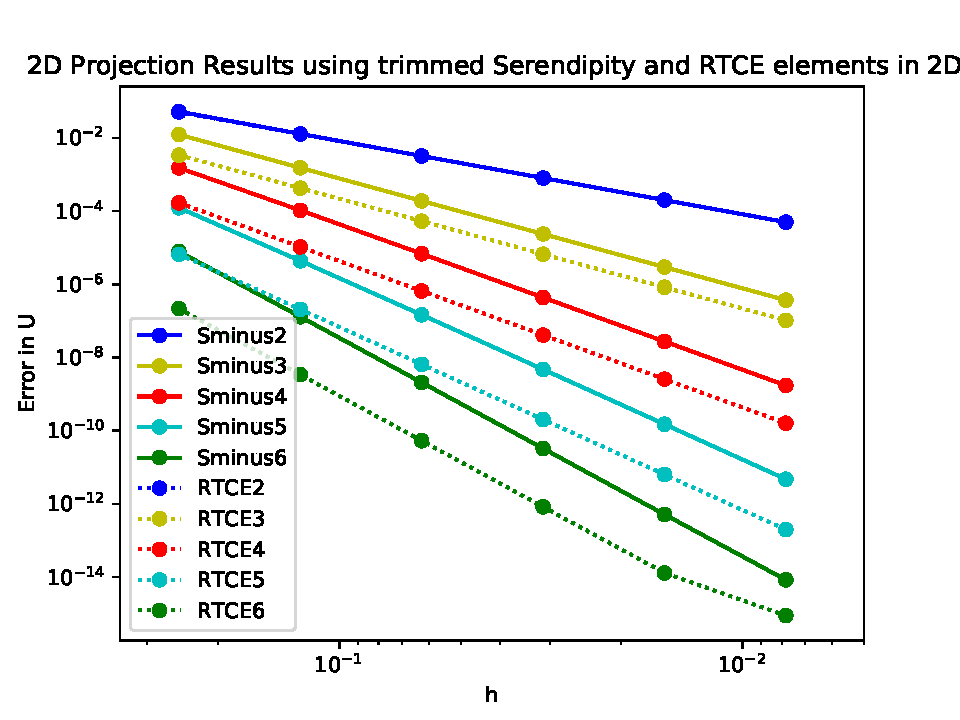
\includegraphics[height=2.2in]{2dProjectionH.pdf}
    \begin{tikzpicture}[scale=0.88]
      \begin{loglogaxis}[xlabel={h}, ylabel={Error},
             ylabel near ticks, ymax=1e-1, ymin=2e-11, xmax=0.3, xmin=0.5e-2,
             legend pos=south east, legend style={font=\tiny} ,
             cycle list name=color list, title={Projection Error Analysis in 2D}]
        %\addplot+[only marks, orange] table [x=Dofs,y=Time,col sep=comma]{PrimalPoissonSerendipity3dO4.csv};
        \addplot[red]
        table [x=h,y=Error, col sep=comma]{csvs/ProjectionSminus2dO2.csv};
        \addlegendentry{$S^-_2$}
        \addplot[blue] 
        table [x=h,y=Error, col sep=comma]{csvs/ProjectionSminus2dO3.csv};
        \addlegendentry{$S^-_3$ }
        \addplot[orange]
        table [x=h,y=Error, col sep=comma]{csvs/ProjectionSminus2dO4.csv};
        \addlegendentry{$S^-_4$}
        \addplot[densely dotted, red]
        table [x=h,y=Error, col sep=comma]{csvs/ProjectionRTCE2dO2.csv};
        \addlegendentry{$Q^-_2$}
        \addplot[densely dotted, blue] 
        table [x=h,y=Error, col sep=comma]{csvs/ProjectionRTCE2dO3.csv};
        \addlegendentry{$Q^-_3$}
        \addplot[densely dotted, orange]
        table [x=h,y=Error, col sep=comma]{csvs/ProjectionRTCE2dO4.csv};
        \addlegendentry{$Q^-_4$}
        
        \addplot+[only marks, red] table [x=h,y=Error,col sep=comma]{csvs/ProjectionSminus2dO2.csv};
        \addplot+[only marks, red, mark=square*] table [x=h,y=Error,col sep=comma]{csvs/ProjectionRTCE2dO2.csv};
        \addplot+[only marks, blue] table [x=h,y=Error,col sep=comma]{csvs/ProjectionSminus2dO3.csv};
        \addplot+[only marks, blue, mark=square*] table [x=h,y=Error,col sep=comma]{csvs/ProjectionRTCE2dO3.csv};
        \addplot+[only marks, orange] table [x=h,y=Error,col sep=comma]{csvs/ProjectionSminus2dO4.csv};
        \addplot+[only marks, orange, mark=square*] table [x=h,y=Error,col sep=comma]{csvs/ProjectionRTCE2dO4.csv};
      \end{loglogaxis}
      \end{tikzpicture}
    \caption{2D edge length vs error}
    \label{fig:2dProjectionH}
  \end{subfigure}
  ~
  \begin{subfigure}[h]{0.5\textwidth}
     %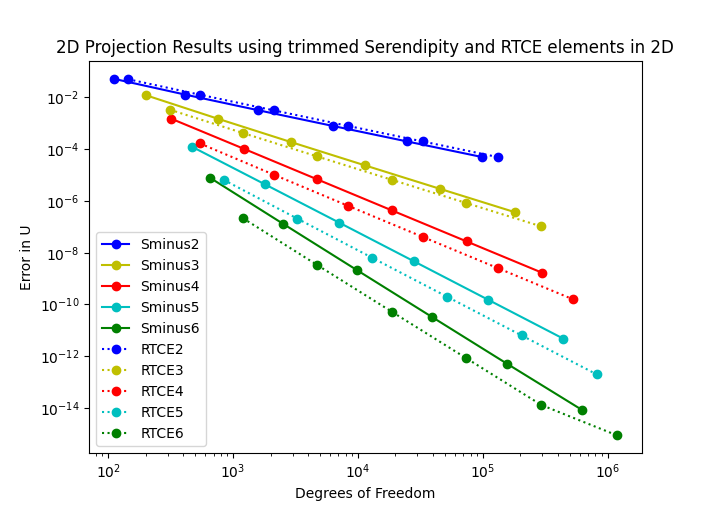
\includegraphics[height=2.2in]{2dProjection.png}
     \begin{tikzpicture}[scale=0.88]
      \begin{loglogaxis}[xlabel={Degrees of Freedom}, ylabel={Error},
             ylabel near ticks, ymax=1e-1, ymin=2e-11, xmax=3e6, xmin=0.5e2,
             legend pos=south west, legend style={font=\tiny} ,
             cycle list name=color list, title={Projection Error Analysis in 2D}]
        %\addplot+[only marks, orange] table [x=Dofs,y=Time,col sep=comma]{PrimalPoissonSerendipity3dO4.csv};
        \addplot[red]
        table [x=Dofs,y=Error, col sep=comma]{csvs/ProjectionSminus2dO2.csv};
        \addlegendentry{$S^-_2$}
        \addplot[blue] 
        table [x=Dofs,y=Error, col sep=comma]{csvs/ProjectionSminus2dO3.csv};
        \addlegendentry{$S^-_3$ }
        \addplot[orange]
        table [x=Dofs,y=Error, col sep=comma]{csvs/ProjectionSminus2dO4.csv};
        \addlegendentry{$S^-_4$}
        \addplot[densely dotted, red]
        table [x=Dofs,y=Error, col sep=comma]{csvs/ProjectionRTCE2dO2.csv};
        \addlegendentry{$Q^-_2$}
        \addplot[densely dotted, blue] 
        table [x=Dofs,y=Error, col sep=comma]{csvs/ProjectionRTCE2dO3.csv};
        \addlegendentry{$Q^-_3$}
        \addplot[densely dotted, orange]
        table [x=Dofs,y=Error, col sep=comma]{csvs/ProjectionRTCE2dO4.csv};
        \addlegendentry{$Q^-_4$}
        
        \addplot+[only marks, red] table [x=Dofs,y=Error,col sep=comma]{csvs/ProjectionSminus2dO2.csv};
        \addplot+[only marks, red, mark=square*] table [x=Dofs,y=Error,col sep=comma]{csvs/ProjectionRTCE2dO2.csv};
        \addplot+[only marks, blue] table [x=Dofs,y=Error,col sep=comma]{csvs/ProjectionSminus2dO3.csv};
        \addplot+[only marks, blue, mark=square*] table [x=Dofs,y=Error,col sep=comma]{csvs/ProjectionRTCE2dO3.csv};
        \addplot+[only marks, orange] table [x=Dofs,y=Error,col sep=comma]{csvs/ProjectionSminus2dO4.csv};
        \addplot+[only marks, orange, mark=square*] table [x=Dofs,y=Error,col sep=comma]{csvs/ProjectionRTCE2dO4.csv};
      \end{loglogaxis}
      \end{tikzpicture}
     \caption{2D degrees of freedom vs error}
     \label{fig:2dProjection}
  \end{subfigure} \\
  ~
  \begin{subfigure}[h]{0.5\textwidth}
    \begin{tikzpicture}[scale=0.88]
      \begin{loglogaxis}[xlabel={h}, ylabel={Error},
             ylabel near ticks, ymax=1e-1, ymin=2e-10, xmax=0.2, xmin=0.5e-2,
             legend pos=south east, legend style={font=\tiny} ,
             cycle list name=color list, title={Projection Error Analysis in 3D}]
        %\addplot+[only marks, orange] table [x=Dofs,y=Time,col sep=comma]{PrimalPoissonSerendipity3dO4.csv};
        \addplot[red]
        table [x=h,y=Error, col sep=comma]{csvs/ProjectionSminus3dO2.csv};
        \addlegendentry{$S^-_2$}
        \addplot[blue] 
        table [x=h,y=Error, col sep=comma]{csvs/ProjectionSminus3dO3.csv};
        \addlegendentry{$S^-_3$ }
        \addplot[orange]
        table [x=h,y=Error, col sep=comma]{csvs/ProjectionSminus3dO4.csv};
        \addlegendentry{$S^-_4$}
        \addplot[densely dotted, red]
        table [x=h,y=Error, col sep=comma]{csvs/ProjectionNCE3dO2.csv};
        \addlegendentry{$Q^-_2$}
        \addplot[densely dotted, blue] 
        table [x=h,y=Error, col sep=comma]{csvs/ProjectionNCE3dO3.csv};
        \addlegendentry{$Q^-_3$}
        \addplot[densely dotted, orange]
        table [x=h,y=Error, col sep=comma]{csvs/ProjectionNCE3dO4.csv};
        \addlegendentry{$Q^-_4$}
        
        \addplot+[only marks, red] table [x=h,y=Error,col sep=comma]{csvs/ProjectionSminus3dO2.csv};
        \addplot+[only marks, red, mark=square*] table [x=h,y=Error,col sep=comma]{csvs/ProjectionNCE3dO2.csv};
        \addplot+[only marks, blue] table [x=h,y=Error,col sep=comma]{csvs/ProjectionSminus3dO3.csv};
        \addplot+[only marks, blue, mark=square*] table [x=h,y=Error,col sep=comma]{csvs/ProjectionNCE3dO3.csv};
        \addplot+[only marks, orange] table [x=h,y=Error,col sep=comma]{csvs/ProjectionSminus3dO4.csv};
        \addplot+[only marks, orange, mark=square*] table [x=h,y=Error,col sep=comma]{csvs/ProjectionNCE3dO4.csv};
      \end{loglogaxis}
      \end{tikzpicture}
    %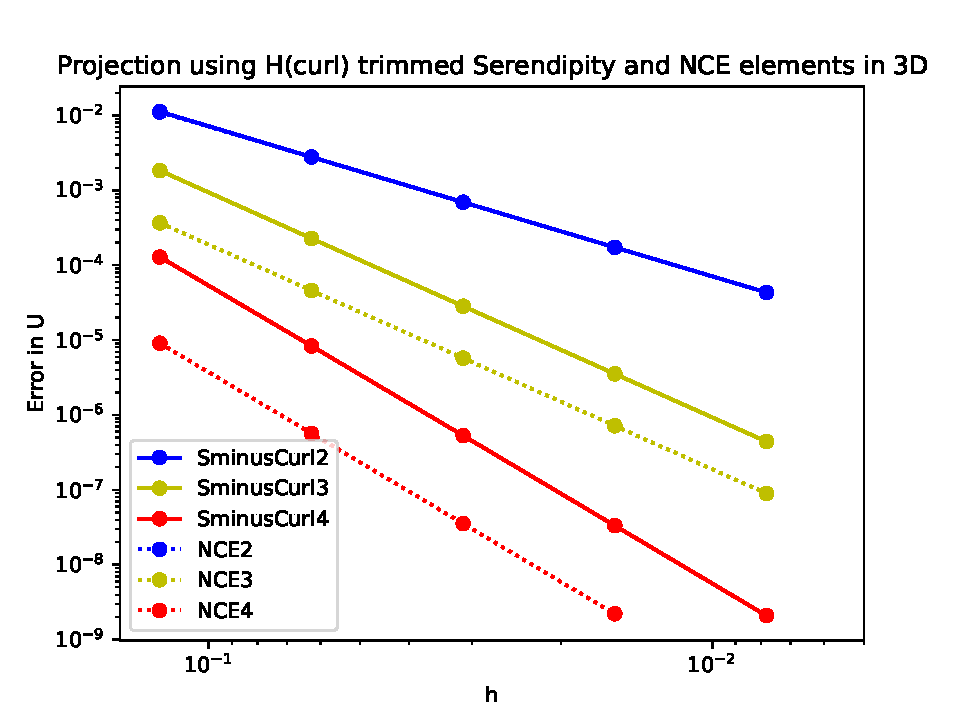
\includegraphics[height=2.2in]{3dProjectionHError.pdf}
    \caption{3D edge length vs error}
    \label{fig:3dProjectionH}
  \end{subfigure}
  ~
  \begin{subfigure}[h]{0.5\textwidth}
  \begin{tikzpicture}[scale=0.88]
      \begin{loglogaxis}[xlabel={Degrees of Freedom}, ylabel={Error},
             ylabel near ticks, ymax=3e-2, ymin=0.5e-9, xmax=4e8, xmin=0.25e4,
             legend pos=south west, legend style={font=\tiny} ,
             cycle list name=color list, title={Projection Error Analysis in 3D}]
        %\addplot+[only marks, orange] table [x=Dofs,y=Time,col sep=comma]{PrimalPoissonSerendipity3dO4.csv};
        \addplot[red]
        table [x=Dofs,y=Error, col sep=comma]{csvs/ProjectionSminus3dO2.csv};
        \addlegendentry{$S^-_2$}
        \addplot[blue] 
        table [x=Dofs,y=Error, col sep=comma]{csvs/ProjectionSminus3dO3.csv};
        \addlegendentry{$S^-_3$ }
        \addplot[orange]
        table [x=Dofs,y=Error, col sep=comma]{csvs/ProjectionSminus3dO4.csv};
        \addlegendentry{$S^-_4$}
        \addplot[densely dotted, red]
        table [x=Dofs,y=Error, col sep=comma]{csvs/ProjectionNCE3dO2.csv};
        \addlegendentry{$Q^-_2$}
        \addplot[densely dotted, blue] 
        table [x=Dofs,y=Error, col sep=comma]{csvs/ProjectionNCE3dO3.csv};
        \addlegendentry{$Q^-_3$}
        \addplot[densely dotted, orange]
        table [x=Dofs,y=Error, col sep=comma]{csvs/ProjectionNCE3dO4.csv};
        \addlegendentry{$Q^-_4$}
        
        \addplot+[only marks, red] table [x=Dofs,y=Error,col sep=comma]{csvs/ProjectionSminus3dO2.csv};
        \addplot+[only marks, red, mark=square*] table [x=Dofs,y=Error,col sep=comma]{csvs/ProjectionNCE3dO2.csv};
        \addplot+[only marks, blue] table [x=Dofs,y=Error,col sep=comma]{csvs/ProjectionSminus3dO3.csv};
        \addplot+[only marks, blue, mark=square*] table [x=Dofs,y=Error,col sep=comma]{csvs/ProjectionNCE3dO3.csv};
        \addplot+[only marks, orange] table [x=Dofs,y=Error,col sep=comma]{csvs/ProjectionSminus3dO4.csv};
        \addplot+[only marks, orange, mark=square*] table [x=Dofs,y=Error,col sep=comma]{csvs/ProjectionNCE3dO4.csv};
      \end{loglogaxis}
      \end{tikzpicture}
    %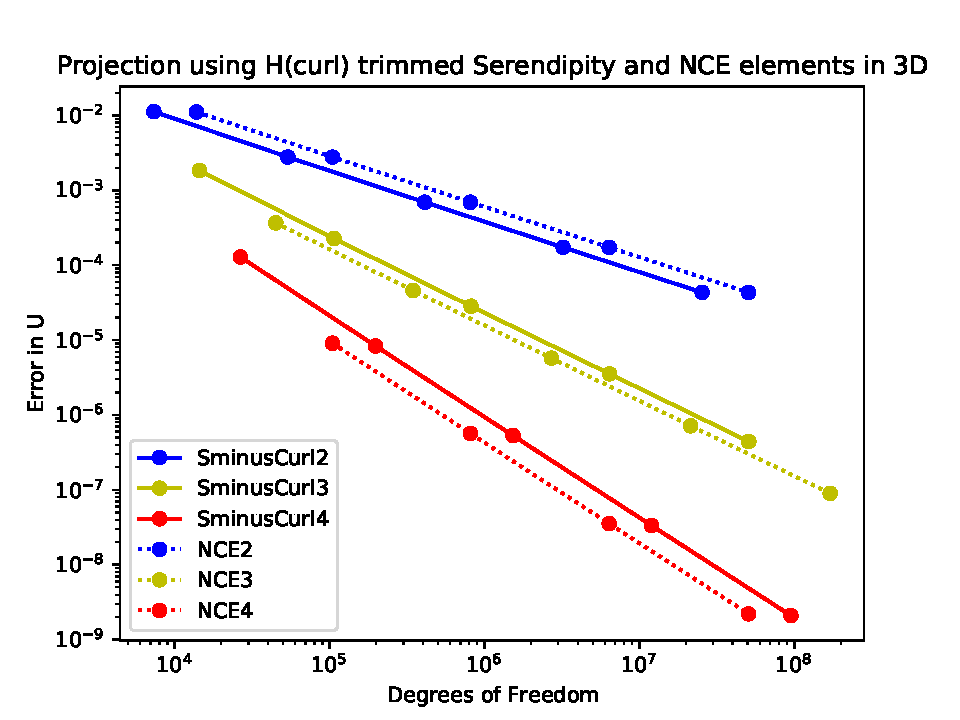
\includegraphics[height=2.2in]{3dProjectionDofsError.pdf}
    \caption{3D degrees of freedom vs error}
    \label{fig:3dProjectionDofs}
  \end{subfigure}
  \caption{Results of solving projection problem using 2D and 3D $S^-$ curl elements and tensor product curl elements.}
\end{figure}
  
First, we graphed the errors from computing projections using trimmed Serendipity and tensor product elements in 2D, shown in Figure \ref{fig:2dProjectionH}.  Since we expect that the order of convergence for both of these elements should be the same (only off by a constant factor), we look for the lines representing trimmed Serendipity and tensor product elements at a given order to be parallel.
  
After checking that it is converging at the right rate, we then want to analyze the data from a standpoint of memory usage.  To do this, we plot degrees of freedom vs error, as seen in Figure \ref{fig:2dProjection}.  Overall, the error given by trimmed Serendipity elements is higher than the error from using tensor product elements of the same order.   We see similar results in Figures \ref{fig:3dProjectionDofs} and \ref{fig:3dProjectionH}.
  


\newpage
 
\subsection{The Poisson Problem}
In this section we discuss results for both the primal Poisson problem as well as the mixed Poisson problem.  We solve the primal Poisson problem described below on a unit square domain $\Omega$:
\begin{align}
    -\nabla^2 u &= f \\
    u\vert_{\partial \Omega} &= 0 \\
    \nabla u \cdot n &= 0 \text{ on } \partial \Omega
\end{align}
where $f(x,y) = 2\pi^2\text{sin}(\pi x)\text{sin}(\pi y) $, yielding the solution $u(x,y) = \text{sin}(\pi x)\text{sin}(\pi y)$. In 3D, we can extend this to $f(x,y,z) = 2\pi^2\text{sin}(\pi x)\text{sin}(\pi y)\text{sin}(\pi z)$ with the solution being $u(x,y,z) = \text{sin}(\pi x)\text{sin}(\pi y)\text{sin}(\pi z)$.  

The primal Poisson problem allows us to test scalar Serendipity elements against Lagrange elements.  Then we wish to also test H(div) elements.  To do this, we solve a discretization of the mixed Poisson problem:

\begin{align}
     \sigma - \nabla u &= 0 \\
     \nabla \cdot \sigma &= -f \notag \\
     u\vert_{\partial \Omega} &= 0 \notag
\end{align}


\begin{figure}[h!]
  \centering
  \begin{subfigure}[h]{0.5\textwidth}
    \centering
      \begin{tikzpicture}[scale=0.88]
      \begin{loglogaxis}[xlabel={Degrees of Freedom}, ylabel={Error},
             ylabel near ticks, ymax=1e-4, ymin=1e-16, xmax=2e6, xmin=2e3,
             legend pos=south west, legend style={font=\tiny} ,
             cycle list name=color list, title={Primal Poisson Error Analysis}]
        %\addplot+[only marks, orange] table [x=Dofs,y=Time,col sep=comma]{PrimalPoissonSerendipity3dO4.csv};
        \addplot[red]
        table [x=Dofs,y=Error, col sep=comma]{csvs/PrimalPoissonSerendipity2dO2.csv};
        \addlegendentry{$S^-_2$}
        \addplot[blue] 
        table [x=Dofs,y=Error, col sep=comma]{csvs/PrimalPoissonSerendipity2dO3.csv};
        \addlegendentry{$S^-_3$ }
        \addplot[orange]
        table [x=Dofs,y=Error, col sep=comma]{csvs/PrimalPoissonSerendipity2dO4.csv};
        \addlegendentry{$S^-_4$}
        \addplot[densely dotted, red]
        table [x=Dofs,y=Error, col sep=comma]{csvs/PrimalPoissonLagrange2dO2.csv};
        \addlegendentry{$Q^-_2$}
        \addplot[densely dotted, blue] 
        table [x=Dofs,y=Error, col sep=comma]{csvs/PrimalPoissonLagrange2dO3.csv};
        \addlegendentry{$Q^-_3$}
        \addplot[densely dotted, orange]
        table [x=Dofs,y=Error, col sep=comma]{csvs/PrimalPoissonLagrange2dO4.csv};
        \addlegendentry{$Q^-_4$}
        
        \addplot+[only marks, red] table [x=Dofs,y=Error,col sep=comma]{csvs/PrimalPoissonSerendipity2dO2.csv};
        \addplot+[only marks, red, mark=square*] table [x=Dofs,y=Error,col sep=comma]{csvs/PrimalPoissonLagrange2dO2.csv};
        \addplot+[only marks, blue] table [x=Dofs,y=Error,col sep=comma]{csvs/PrimalPoissonSerendipity2dO3.csv};
        \addplot+[only marks, blue, mark=square*] table [x=Dofs,y=Error,col sep=comma]{csvs/PrimalPoissonLagrange2dO3.csv};
        \addplot+[only marks, orange] table [x=Dofs,y=Error,col sep=comma]{csvs/PrimalPoissonSerendipity2dO4.csv};
        \addplot+[only marks, orange, mark=square*] table [x=Dofs,y=Error,col sep=comma]{csvs/PrimalPoissonLagrange2dO4.csv};
      \end{loglogaxis}
      \end{tikzpicture}
    %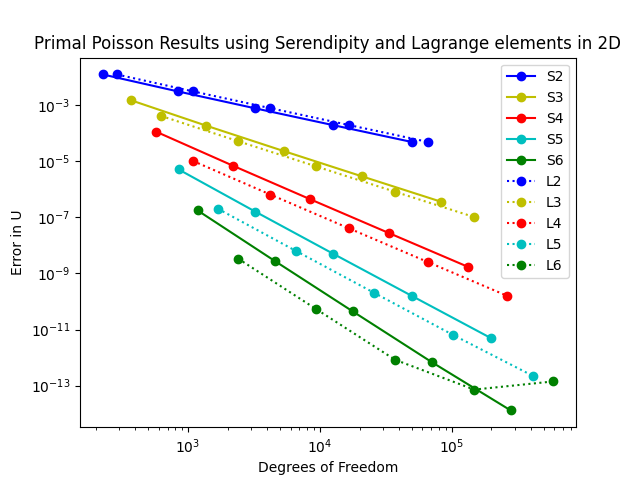
\includegraphics[height=2.2in]{2dPrimalPoisson.png}
    \caption{2D Primal}
    \label{fig:2dPrimalDofs}
  \end{subfigure}
  ~
  \begin{subfigure}[h]{0.5\textwidth}
    \centering
    \begin{tikzpicture}[scale=0.88]
      \begin{loglogaxis}[xlabel={Degrees of Freedom}, ylabel={Error},
             ylabel near ticks, ymax=1e-1, ymin=1e-11, xmax=2e6, xmin=3e2,
             legend pos=south west, legend style={font=\tiny} ,
             cycle list name=color list, title={Mixed Poisson Error Analysis}]
        %\addplot+[only marks, orange] table [x=Dofs,y=Time,col sep=comma]{PrimalPoissonSerendipity3dO4.csv};
        \addplot[red]
        table [x=Dofs,y=Error, col sep=comma]{csvs/MixedPoissonSminus2dO2.csv};
        \addlegendentry{$S^-_2$}
        \addplot[blue] 
        table [x=Dofs,y=Error, col sep=comma]{csvs/MixedPoissonSminus2dO3.csv};
        \addlegendentry{$S^-_3$ }
        \addplot[orange]
        table [x=Dofs,y=Error, col sep=comma]{csvs/MixedPoissonSminus2dO4.csv};
        \addlegendentry{$S^-_4$}
        \addplot[densely dotted, red]
        table [x=Dofs,y=Error, col sep=comma]{csvs/MixedPoissonRTCF2dO2.csv};
        \addlegendentry{$Q^-_2$}
        \addplot[densely dotted, blue] 
        table [x=Dofs,y=Error, col sep=comma]{csvs/MixedPoissonRTCF2dO3.csv};
        \addlegendentry{$Q^-_3$}
        \addplot[densely dotted, orange]
        table [x=Dofs,y=Error, col sep=comma]{csvs/MixedPoissonRTCF2dO4.csv};
        \addlegendentry{$Q^-_4$}
        
        \addplot+[only marks, red] table [x=Dofs,y=Error,col sep=comma]{csvs/MixedPoissonSminus2dO2.csv};
        \addplot+[only marks, red, mark=square*] table [x=Dofs,y=Error,col sep=comma]{csvs/MixedPoissonRTCF2dO2.csv};
        \addplot+[only marks, blue] table [x=Dofs,y=Error,col sep=comma]{csvs/MixedPoissonSminus2dO3.csv};
        \addplot+[only marks, blue, mark=square*] table [x=Dofs,y=Error,col sep=comma]{csvs/MixedPoissonRTCF2dO3.csv};
        \addplot+[only marks, orange] table [x=Dofs,y=Error,col sep=comma]{csvs/MixedPoissonSminus2dO4.csv};
        \addplot+[only marks, orange, mark=square*] table [x=Dofs,y=Error,col sep=comma]{csvs/MixedPoissonRTCF2dO4.csv};
      \end{loglogaxis}
      \end{tikzpicture}
    %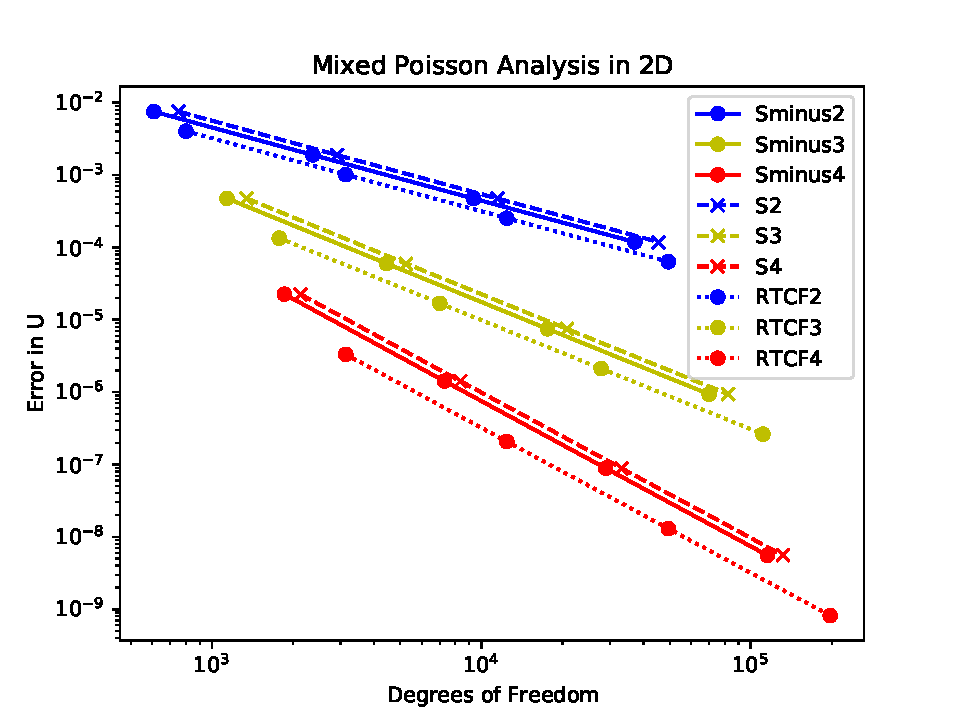
\includegraphics[height=2.2in]{2dMixedPoissonDofs.pdf}
    \caption{2D Mixed}
    \label{fig:2dMixedDofsError}
  \end{subfigure} \\
  \begin{subfigure}[h]{0.5\textwidth}
    \centering
    \begin{tikzpicture}[scale=0.88]
      \begin{loglogaxis}[xlabel={Degrees of Freedom}, ylabel={Error},
             ylabel near ticks, ymax=1e-3, ymin=1e-11, xmax=2e8, xmin=1e3,
             legend pos=south west, legend style={font=\tiny} ,
             cycle list name=color list, title={Primal Poisson Error Analysis}]
        %\addplot+[only marks, orange] table [x=Dofs,y=Time,col sep=comma]{PrimalPoissonSerendipity3dO4.csv};
        \addplot[red]
        table [x=Dofs,y=Error, col sep=comma]{csvs/PrimalPoissonSerendipity3dO2.csv};
        \addlegendentry{$S^-_2$}
        \addplot[blue] 
        table [x=Dofs,y=Error, col sep=comma]{csvs/PrimalPoissonSerendipity3dO3.csv};
        \addlegendentry{$S^-_3$ }
        \addplot[orange]
        table [x=Dofs,y=Error, col sep=comma]{csvs/PrimalPoissonSerendipity3dO4.csv};
        \addlegendentry{$S^-_4$}
        \addplot[densely dotted, red]
        table [x=Dofs,y=Error, col sep=comma]{csvs/PrimalPoissonLagrange3dO2.csv};
        \addlegendentry{$Q^-_2$}
        \addplot[densely dotted, blue] 
        table [x=Dofs,y=Error, col sep=comma]{csvs/PrimalPoissonLagrange3dO3.csv};
        \addlegendentry{$Q^-_3$}
        \addplot[densely dotted, orange]
        table [x=Dofs,y=Error, col sep=comma]{csvs/PrimalPoissonLagrange3dO4.csv};
        \addlegendentry{$Q^-_4$}
        
        \addplot+[only marks, red] table [x=Dofs,y=Error,col sep=comma]{csvs/PrimalPoissonSerendipity3dO2.csv};
        \addplot+[only marks, red, mark=square*] table [x=Dofs,y=Error,col sep=comma]{csvs/PrimalPoissonLagrange3dO2.csv};
        \addplot+[only marks, blue] table [x=Dofs,y=Error,col sep=comma]{csvs/PrimalPoissonSerendipity3dO3.csv};
        \addplot+[only marks, blue, mark=square*] table [x=Dofs,y=Error,col sep=comma]{csvs/PrimalPoissonLagrange3dO3.csv};
        \addplot+[only marks, orange] table [x=Dofs,y=Error,col sep=comma]{csvs/PrimalPoissonSerendipity3dO4.csv};
        \addplot+[only marks, orange, mark=square*] table [x=Dofs,y=Error,col sep=comma]{csvs/PrimalPoissonLagrange3dO4.csv};
      \end{loglogaxis}
      \end{tikzpicture}
    %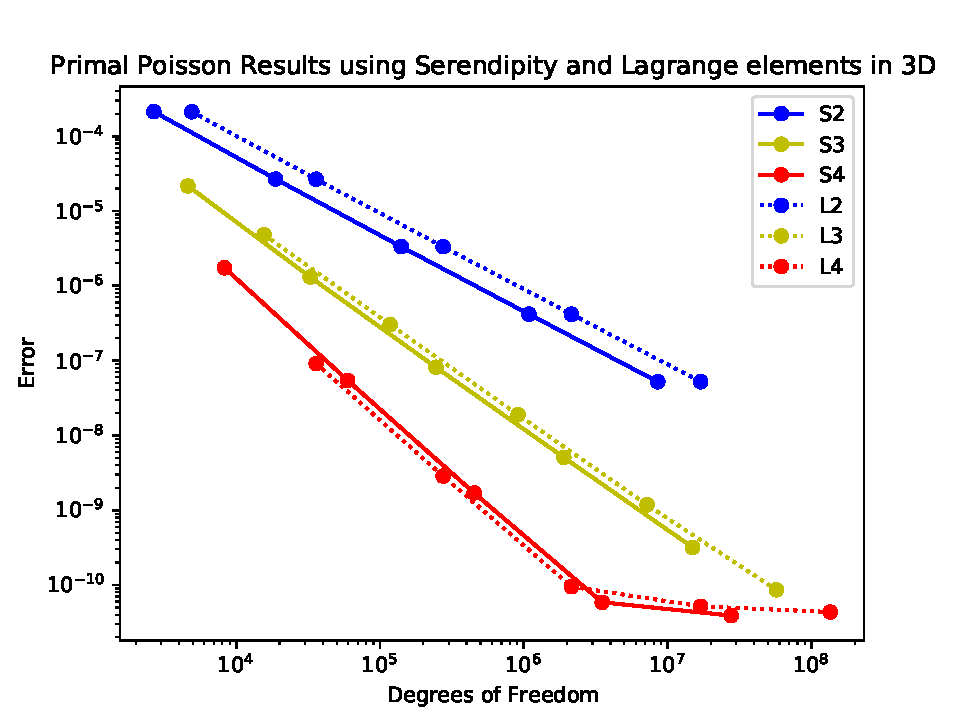
\includegraphics[height=2.2in]{3dPrimalDofsError.pdf}
    \caption{3D Primal}
    \label{fig:3dPrimalDofsError}
  \end{subfigure}
  ~
  \begin{subfigure}[h]{0.5\textwidth}
    \centering
    %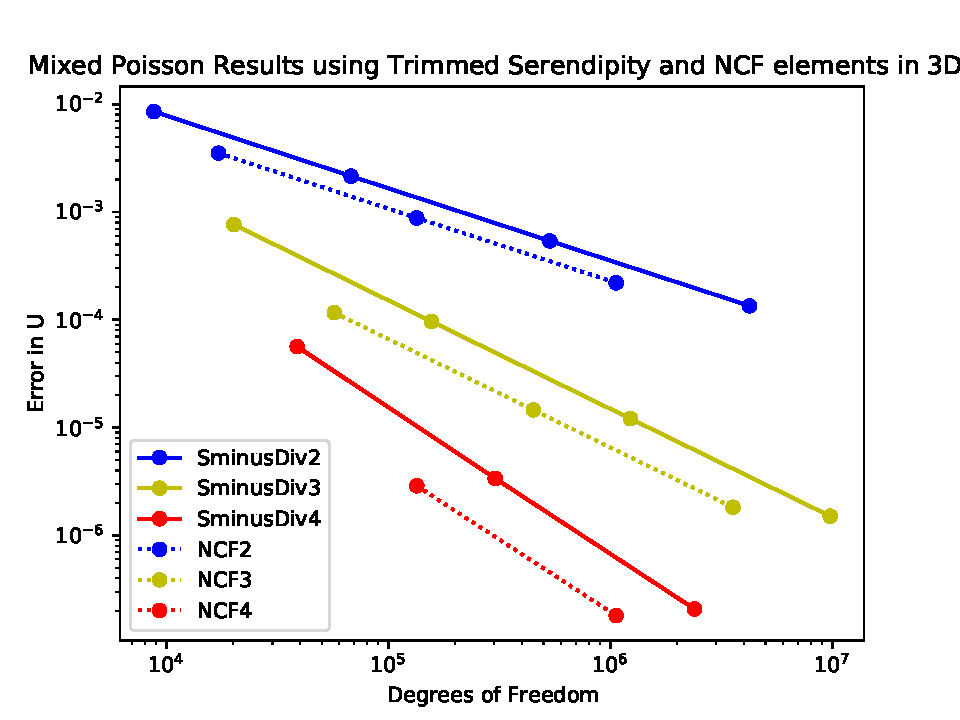
\includegraphics[height=2.2in]{3dMixedPoissonDofsError.pdf}
    \begin{tikzpicture}[scale=0.88]
      \begin{loglogaxis}[xlabel={Degrees of Freedom}, ylabel={Error},
             ylabel near ticks, ymax=1.2e-2, ymin=0.8e-7, xmax=2e7, xmin=5e3,
             legend pos=south west, legend style={font=\tiny} ,
             cycle list name=color list, title={Mixed Poisson Error Analysis}]
        %\addplot+[only marks, orange] table [x=Dofs,y=Time,col sep=comma]{PrimalPoissonSerendipity3dO4.csv};
        \addplot[red]
        table [x=Dofs,y=Error, col sep=comma]{csvs/MixedPoissonSminus3dO2.csv};
        \addlegendentry{$S^-_2$}
        \addplot[blue] 
        table [x=Dofs,y=Error, col sep=comma]{csvs/MixedPoissonSminus3dO3.csv};
        \addlegendentry{$S^-_3$ }
        \addplot[orange]
        table [x=Dofs,y=Error, col sep=comma]{csvs/MixedPoissonSminus3dO4.csv};
        \addlegendentry{$S^-_4$}
        \addplot[densely dotted, red]
        table [x=Dofs,y=Error, col sep=comma]{csvs/MixedPoissonNCF3dO2.csv};
        \addlegendentry{$Q^-_2$}
        \addplot[densely dotted, blue] 
        table [x=Dofs,y=Error, col sep=comma]{csvs/MixedPoissonNCF3dO3.csv};
        \addlegendentry{$Q^-_3$}
        \addplot[densely dotted, orange]
        table [x=Dofs,y=Error, col sep=comma]{csvs/MixedPoissonNCF3dO4.csv};
        \addlegendentry{$Q^-_4$}
        
        \addplot+[only marks, red] table [x=Dofs,y=Error,col sep=comma]{csvs/MixedPoissonSminus3dO2.csv};
        \addplot+[only marks, red, mark=square*] table [x=Dofs,y=Error,col sep=comma]{csvs/MixedPoissonNCF3dO2.csv};
        \addplot+[only marks, blue] table [x=Dofs,y=Error,col sep=comma]{csvs/MixedPoissonSminus3dO3.csv};
        \addplot+[only marks, blue, mark=square*] table [x=Dofs,y=Error,col sep=comma]{csvs/MixedPoissonNCF3dO3.csv};
        \addplot+[only marks, orange] table [x=Dofs,y=Error,col sep=comma]{csvs/MixedPoissonSminus3dO4.csv};
        \addplot+[only marks, orange, mark=square*] table [x=Dofs,y=Error,col sep=comma]{csvs/MixedPoissonNCF3dO4.csv};
      \end{loglogaxis}
      \end{tikzpicture}
    \caption{3D Mixed}
    \label{fig:3dMixedDofsError}
  \end{subfigure}
  \caption{An error analysis of the primal and mixed Poisson problems in 2D and 3D.}
\label{fig:PrimalMixedErrorAnalysis}
\end{figure}


Figures \ref{fig:2dPrimalDofs}, \ref{fig:2dMixedDofsError}, \ref{fig:3dPrimalDofsError}, and \ref{fig:3dMixedDofsError} give us some interesting data points to focus on.  Before analyzing the results, note again that Serendipity and trimmed Serendipity elements are the same in the primal Poisson case.  While these elements differ in the H(div) and H(curl) cases, our results here indicate that we likely will not see Serendiptiy elements outperforming trimmed Serendipity elements in 3D, so their implementation has been left for a future work.

In each of the figures in \ref{fig:PrimalMixedErrorAnalysis}, we see that regardless of which element is better, they follow similar trajectories again, indicating that they have the same overall convergence rate.  The primal Poisson problem shows us that there are scenarios where using Serendipity elements can be beneficial in terms of error depending on the number of degrees of freedom.  However, in the mixed Poisson problem, we don't immediately see this benefit in either the 2D case or the 3D case.

However, we would also like to analyze timing for tensor product elements and trimmed Serendipity elements.  We do this in the subfigures of \ref{fig:PrimalMixedTimeAnalysis}.  In \ref{fig:3dPrimalDofsTime} and \ref{fig:3dPrimalTimeError}, we see good evidence that Serendipity elements are able to to produce better results at a faster rate.  Specifically, in \ref{fig:3dPrimalDofsTime}, we can see that Serendipity elements are able to do a larger number of degrees of freedom in the same amount of time.  In fig \ref{fig:3dPrimalTimeError} we see that for a given error level, Serendipity elements require less time.

However the picture that is painted in \ref{fig:3dMixedDofsTime} and \ref{fig:3dMixedTimeError} is much less clear.  Overall, trimmed Serendipity elements seem to do a bit worse than the corresponding tensor product elements for the mixed Poisson problem, but it is promising that in \ref{fig:3dMixedDofsTime}, the points tend to stay in an overall linear fashion bunched together. 

\newpage

\begin{figure}[ht]
  \centering
  \begin{subfigure}[h]{0.5\textwidth}
    \centering
          \begin{tikzpicture}[scale=0.88]
      \begin{loglogaxis}[xlabel={Degrees of Freedom}, ylabel={Time},
             ylabel near ticks, ymax=1.e+4, ymin=0.5e-1, xmax=2.e8, xmin=1.e+3,
             legend pos=north west, legend style={font=\tiny} ,
             cycle list name=color list, title={Primal Poisson using $S^-$ and $Q^-$}]
        %\addplot+[only marks, orange] table [x=Dofs,y=Time,col sep=comma]{PrimalPoissonSerendipity3dO4.csv};
        \addplot[red]
        table [x=Dofs,y=Time, col sep=comma]{csvs/PrimalPoissonSerendipity3dO2.csv};
        \addlegendentry{$S^-_2$}
        \addplot[blue] 
        table [x=Dofs,y=Time, col sep=comma]{csvs/PrimalPoissonSerendipity3dO3.csv};
        \addlegendentry{$S^-_3$ }
        \addplot[orange]
        table [x=Dofs,y=Time, col sep=comma]{csvs/PrimalPoissonSerendipity3dO4.csv};
        \addlegendentry{$S^-_4$}
        \addplot[densely dotted, red]
        table [x=Dofs,y=Time, col sep=comma]{csvs/PrimalPoissonLagrange3dO2.csv};
        \addlegendentry{$Q^-_2$}
        \addplot[densely dotted, blue] 
        table [x=Dofs,y=Time, col sep=comma]{csvs/PrimalPoissonLagrange3dO3.csv};
        \addlegendentry{$Q^-_3$}
        \addplot[densely dotted, orange]
        table [x=Dofs,y=Time, col sep=comma]{csvs/PrimalPoissonLagrange3dO4.csv};
        \addlegendentry{$Q^-_4$}
        
        \addplot+[only marks, red] table [x=Dofs,y=Time,col sep=comma]{csvs/PrimalPoissonSerendipity3dO2.csv};
        \addplot+[only marks, red, mark=square*] table [x=Dofs,y=Time,col sep=comma]{csvs/PrimalPoissonLagrange3dO2.csv};
        \addplot+[only marks, blue] table [x=Dofs,y=Time,col sep=comma]{csvs/PrimalPoissonSerendipity3dO3.csv};
        \addplot+[only marks, blue, mark=square*] table [x=Dofs,y=Time,col sep=comma]{csvs/PrimalPoissonLagrange3dO3.csv};
        \addplot+[only marks, orange] table [x=Dofs,y=Time,col sep=comma]{csvs/PrimalPoissonSerendipity3dO4.csv};
        \addplot+[only marks, orange, mark=square*] table [x=Dofs,y=Time,col sep=comma]{csvs/PrimalPoissonLagrange3dO4.csv};
      \end{loglogaxis}
      \end{tikzpicture}
    %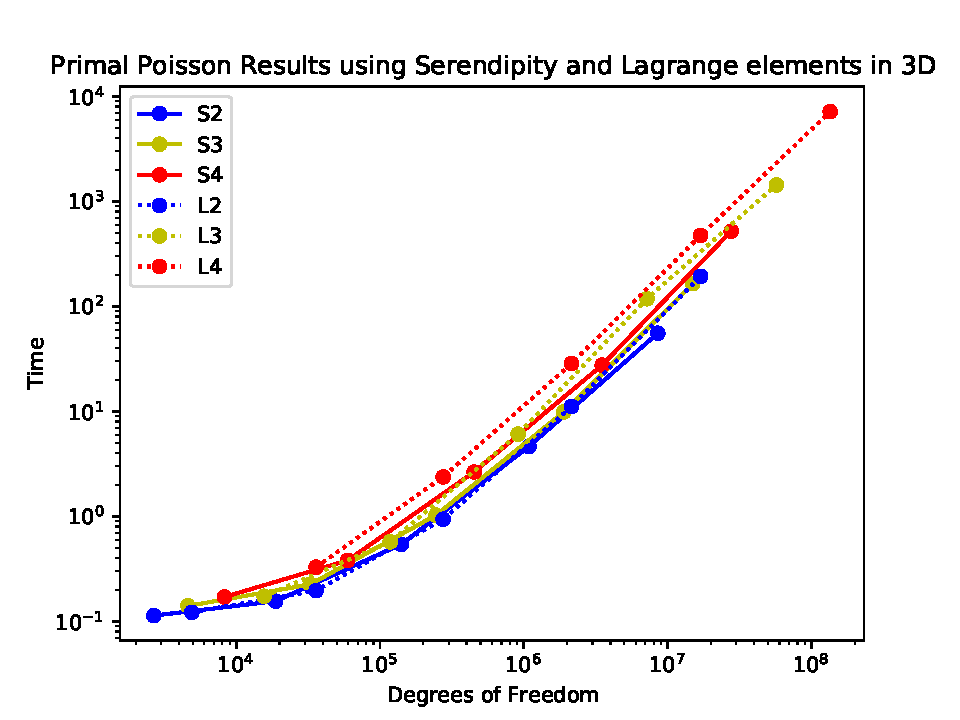
\includegraphics[height=2.2in]{3dPrimalDofsTime.pdf}
    \caption{3D Primal Degrees of freedom vs Time}
    \label{fig:3dPrimalDofsTime}
  \end{subfigure}
  ~
  \begin{subfigure}[h]{0.5\textwidth}
    \centering
    \begin{tikzpicture}[scale=0.88]
      \begin{loglogaxis}[xlabel={Time}, ylabel={Error},
             ylabel near ticks, ymax=1e-3, ymin=1e-11, xmax=1e4, xmin=0.5e-1,
             legend pos=north east, legend style={font=\tiny} ,
             cycle list name=color list, title={Primal Poisson using $S^-$ and $Q^-$}]
        %\addplot+[only marks, orange] table [x=Dofs,y=Time,col sep=comma]{PrimalPoissonSerendipity3dO4.csv};
        \addplot[red]
        table [x=Time,y=Error, col sep=comma]{csvs/PrimalPoissonSerendipity3dO2.csv};
        \addlegendentry{$S^-_2$}
        \addplot[blue] 
        table [x=Time,y=Error, col sep=comma]{csvs/PrimalPoissonSerendipity3dO3.csv};
        \addlegendentry{$S^-_3$ }
        \addplot[orange]
        table [x=Time,y=Error, col sep=comma]{csvs/PrimalPoissonSerendipity3dO4.csv};
        \addlegendentry{$S^-_4$}
        \addplot[densely dotted, red]
        table [x=Time,y=Error, col sep=comma]{csvs/PrimalPoissonLagrange3dO2.csv};
        \addlegendentry{$Q^-_2$}
        \addplot[densely dotted, blue] 
        table [x=Time,y=Error, col sep=comma]{csvs/PrimalPoissonLagrange3dO3.csv};
        \addlegendentry{$Q^-_3$}
        \addplot[densely dotted, orange]
        table [x=Time,y=Error, col sep=comma]{csvs/PrimalPoissonLagrange3dO4.csv};
        \addlegendentry{$Q^-_4$}
        
        \addplot+[only marks, red] table [x=Time,y=Error,col sep=comma]{csvs/PrimalPoissonSerendipity3dO2.csv};
        \addplot+[only marks, red, mark=square*] table [x=Time,y=Error,col sep=comma]{csvs/PrimalPoissonLagrange3dO2.csv};
        \addplot+[only marks, blue] table [x=Time,y=Error,col sep=comma]{csvs/PrimalPoissonSerendipity3dO3.csv};
        \addplot+[only marks, blue, mark=square*] table [x=Time,y=Error,col sep=comma]{csvs/PrimalPoissonLagrange3dO3.csv};
        \addplot+[only marks, orange] table [x=Time,y=Error,col sep=comma]{csvs/PrimalPoissonSerendipity3dO4.csv};
        \addplot+[only marks, orange, mark=square*] table [x=Time,y=Error,col sep=comma]{csvs/PrimalPoissonLagrange3dO4.csv};
      \end{loglogaxis}
      \end{tikzpicture}
    %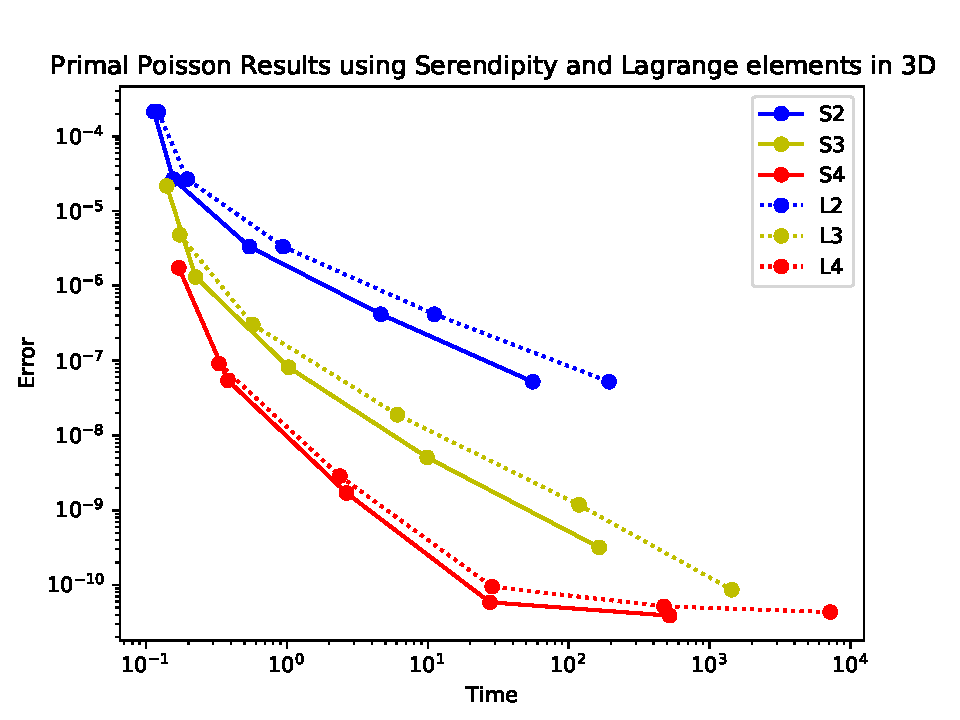
\includegraphics[height=2.2in]{3dPrimalTimeError.pdf}
    \caption{3D Primal Time vs Error}
    \label{fig:3dPrimalTimeError}
  \end{subfigure}\\
  ~
  \begin{subfigure}[h]{0.5\textwidth}
    \centering
    \begin{tikzpicture}[scale=0.88]
      \begin{loglogaxis}[xlabel={Degrees of Freedom}, ylabel={Time},
             ylabel near ticks, ymax=2e4, ymin=1e-1, xmax=2e7, xmin=0.5e4,
             legend pos=north west, legend style={font=\tiny} ,
             cycle list name=color list, title={Mixed Poisson using $S^-$ and $Q^-$}]
        %\addplot+[only marks, orange] table [x=Dofs,y=Time,col sep=comma]{PrimalPoissonSerendipity3dO4.csv};
        \addplot[red]
        table [x=Dofs,y=Time, col sep=comma]{csvs/MixedPoissonSminus3dO2.csv};
        \addlegendentry{$S^-_2$}
        \addplot[blue] 
        table [x=Dofs,y=Time, col sep=comma]{csvs/MixedPoissonSminus3dO3.csv};
        \addlegendentry{$S^-_3$ }
        \addplot[orange]
        table [x=Dofs,y=Time, col sep=comma]{csvs/MixedPoissonSminus3dO4.csv};
        \addlegendentry{$S^-_4$}
        \addplot[densely dotted, red]
        table [x=Dofs,y=Time, col sep=comma]{csvs/MixedPoissonNCF3dO2.csv};
        \addlegendentry{$Q^-_2$}
        \addplot[densely dotted, blue] 
        table [x=Dofs,y=Time, col sep=comma]{csvs/MixedPoissonNCF3dO3.csv};
        \addlegendentry{$Q^-_3$}
        \addplot[densely dotted, orange]
        table [x=Dofs,y=Time, col sep=comma]{csvs/MixedPoissonNCF3dO4.csv};
        \addlegendentry{$Q^-_4$}
        
        \addplot+[only marks, red] table [x=Dofs,y=Time,col sep=comma]{csvs/MixedPoissonSminus3dO2.csv};
        \addplot+[only marks, red, mark=square*] table [x=Dofs,y=Time,col sep=comma]{csvs/MixedPoissonNCF3dO2.csv};
        \addplot+[only marks, blue] table [x=Dofs,y=Time,col sep=comma]{csvs/MixedPoissonSminus3dO3.csv};
        \addplot+[only marks, blue, mark=square*] table [x=Dofs,y=Time,col sep=comma]{csvs/MixedPoissonNCF3dO3.csv};
        \addplot+[only marks, orange] table [x=Dofs,y=Time,col sep=comma]{csvs/MixedPoissonSminus3dO4.csv};
        \addplot+[only marks, orange, mark=square*] table [x=Dofs,y=Time,col sep=comma]{csvs/MixedPoissonNCF3dO4.csv};
      \end{loglogaxis}
      \end{tikzpicture}
    %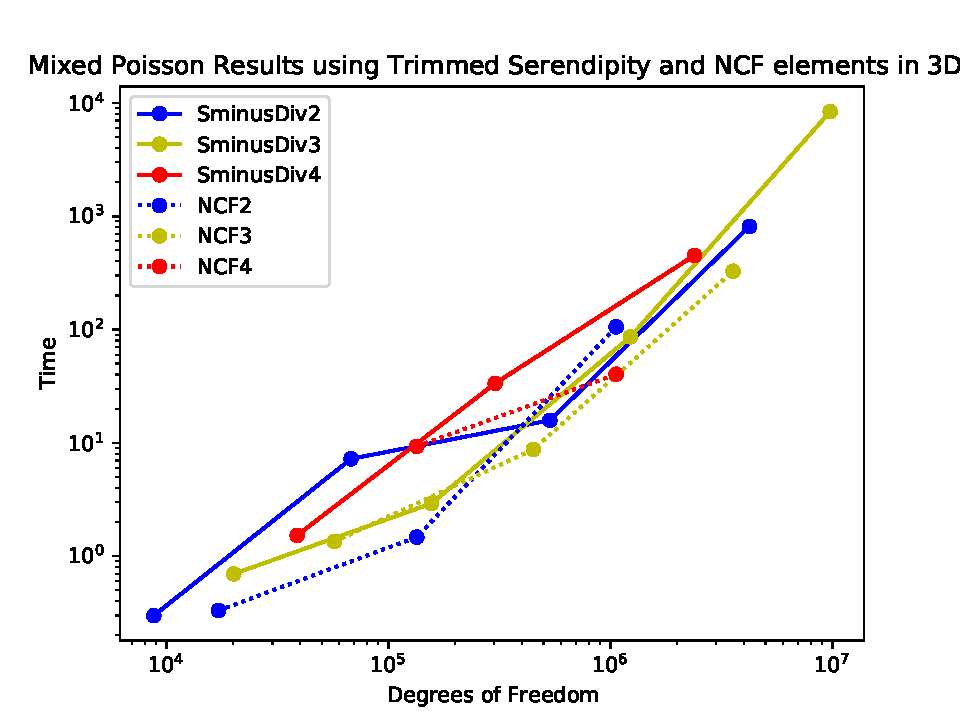
\includegraphics[height=2.2in]{3dMixedPoissonDofsTime.pdf}
    \caption{3D Mixed Degrees of freedom vs Time}
    \label{fig:3dMixedDofsTime}
  \end{subfigure}
  ~
  \begin{subfigure}[h]{0.5\textwidth}
    \centering
    \begin{tikzpicture}[scale=0.88]
      \begin{loglogaxis}[xlabel={Time}, ylabel={Error},
             ylabel near ticks, ymax=1e-1, ymin=5e-8, xmax=1e5, xmin=0.5e-1,
             legend pos=north east, legend style={font=\tiny} ,
             cycle list name=color list, title={Mixed Poisson using $S^-$ and $Q^-$}]
        %\addplot+[only marks, orange] table [x=Dofs,y=Time,col sep=comma]{PrimalPoissonSerendipity3dO4.csv};
        \addplot[red]
        table [x=Time,y=Error, col sep=comma]{csvs/MixedPoissonSminus3dO2.csv};
        \addlegendentry{$S^-_2$}
        \addplot[blue] 
        table [x=Time,y=Error, col sep=comma]{csvs/MixedPoissonSminus3dO3.csv};
        \addlegendentry{$S^-_3$ }
        \addplot[orange]
        table [x=Time,y=Error, col sep=comma]{csvs/MixedPoissonSminus3dO4.csv};
        \addlegendentry{$S^-_4$}
        \addplot[densely dotted, red]
        table [x=Time,y=Error, col sep=comma]{csvs/MixedPoissonNCF3dO2.csv};
        \addlegendentry{$Q^-_2$}
        \addplot[densely dotted, blue] 
        table [x=Time,y=Error, col sep=comma]{csvs/MixedPoissonNCF3dO3.csv};
        \addlegendentry{$Q^-_3$}
        \addplot[densely dotted, orange]
        table [x=Time,y=Error, col sep=comma]{csvs/MixedPoissonNCF3dO4.csv};
        \addlegendentry{$Q^-_4$}
        
        \addplot+[only marks, red] table [x=Time,y=Error,col sep=comma]{csvs/MixedPoissonSminus3dO2.csv};
        \addplot+[only marks, red, mark=square*] table [x=Time,y=Error,col sep=comma]{csvs/MixedPoissonNCF3dO2.csv};
        \addplot+[only marks, blue] table [x=Time,y=Error,col sep=comma]{csvs/MixedPoissonSminus3dO3.csv};
        \addplot+[only marks, blue, mark=square*] table [x=Time,y=Error,col sep=comma]{csvs/MixedPoissonNCF3dO3.csv};
        \addplot+[only marks, orange] table [x=Time,y=Error,col sep=comma]{csvs/MixedPoissonSminus3dO4.csv};
        \addplot+[only marks, orange, mark=square*] table [x=Time,y=Error,col sep=comma]{csvs/MixedPoissonNCF3dO4.csv};
      \end{loglogaxis}
      \end{tikzpicture}
    %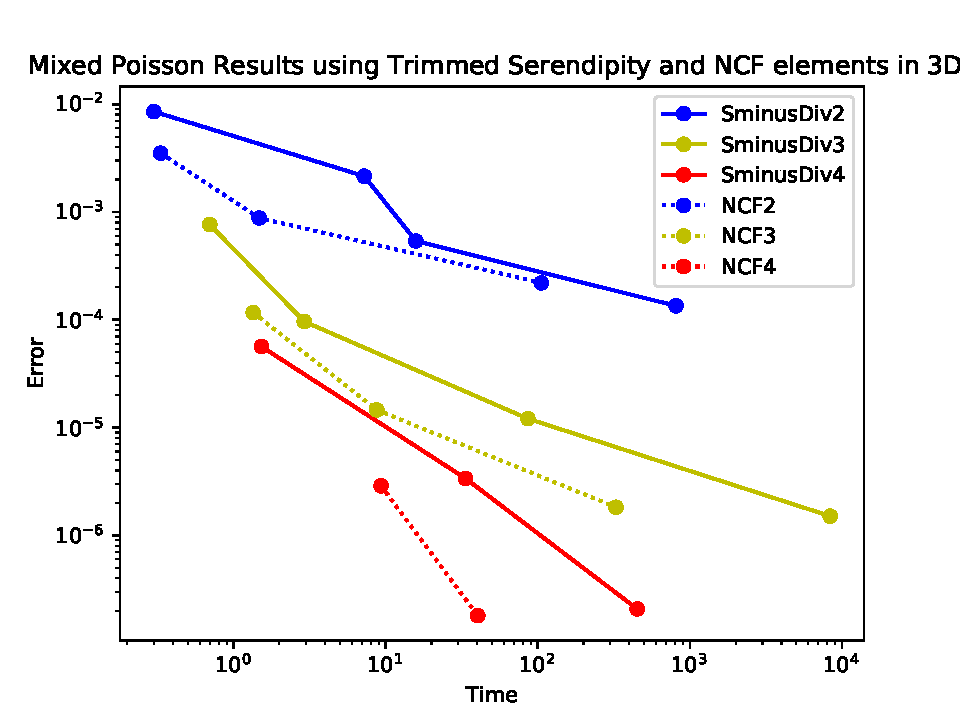
\includegraphics[height=2.2in]{3dMixedPoissonTimeError.pdf}
    \caption{3D Mixed Time vs Error}
    \label{fig:3dMixedTimeError}
  \end{subfigure}
  \caption{Analyzing timing data for primal and mixed Poisson problems using trimmed Serendipity and tensor product elements.}
\label{fig:PrimalMixedTimeAnalysis}
\end{figure}


\newpage  
  
\newpage 



\subsection{Cavity Resonator}

For testing the H$($curl$)$ elements in 3D, we use the cavity resonator problem.  Here, the time-harmonic Maxwell equations are applied to a domain $\Omega = [0,1]^3$ with perfectly conducting boundary conditions, yielding an eigenvalue problem where $\omega$ represents the resonances (i.e.\ eigenvalues) and $E$ represents the electric field (i.e.\ eigenfunctions):


\begin{equation}
    \langle \text{curl}(F), \text{curl}(E) \rangle = \omega^2 \langle F, E \rangle \text{ for all } F \in H_0(\text{curl}).
\end{equation}

%\noindent We tested out the H$($curl$)$ elements in 3D on the cavity resonator problem, where the time-harmonic Maxwell equations applied to a 
%\akg{(1) The wording is a little ambiguous - are you about the state the resonator problem or Maxwell's equations?  Or are these the same?  (2) I prefer to see the statement of the variables prior to the PDE i.e. move the part after the equation to before it. (3) You need to state the domain - I think it's $[0,1]^3\subset\R^3$ - and the boundary conditions (periodic?) (4) Give the eigenvalue equation a label so you can reference it later.}

The exact eigenvalues should follow the formula

\[ \omega^2 = m_1^2 + m_2^2 + m_3^2 \]

\noindent where $m_i \in \mathbb{N} \cup {0}$ and no more than one of $m_1, m_2, m_3$ may be equal to $0$ at a time \cite{rognes2010efficient}.

%\akg{Put discretized version of eigenvalue problem here (see comment below)}

\begin{center}
\begin{table}
\begin{tabular}{ c c c c c }
\multicolumn{5}{c}{NCE Elements} \\
\hline
Actual & N = 4 & N = 8 & N = 16 & N = 32 \\ 
\hline
2 &2.001024 & 2.000066 (3.96) & 2.000004 (4.04) & 2.0000003 (4.00) \\  
2 & 2.001024 & 2.000066 (3.96) & 2.000004 (4.04) & 2.0000003 (4.00)  \\
2 & 2.001024 & 2.000066 (3.96) & 2.000004 (4.04) & 2.0000003 (4.00)\\
3 & 3.001536 & 3.000098 (3.97) & 3.000006 (4.03) & 3.0000004 (4.02) \\
3 & 3.001536 & 3.000098 (3.97) & 3.000006 (4.03) & 3.0000004 (4.02) \\
5 & 5.030601 & 5.002081 (3.88)& 5.000133 (3.97) & 5.000008 (4.06) \\
5 & 5.030601 & 5.002081 (3.88)& 5.000133 (3.97) & 5.000008 (4.06) \\
5 & 5.030601 & 5.002081 (3.88) & 5.000133 (3.97) & 5.000008 (4.06) \\
5 & 5.030601 & 5.0002081 (3.88) & 5.000133 (3.97) & 5.000008 (4.06) \\
6 & 6.031114 & 6.002114 (3.88) & 6.000135 (3.97) &  6.000008 (4.08) \\
6 & 6.031114 & 6.002114 (3.88) & 6.000135 (3.97) & 6.000008 (4.08) \\
6 & 6.031114 & 6.002114 (3.88) & 6.000135 (3.97) & 6.000008 (4.08) \\
8 & - & -& - & - \\
\hline
Iterations & 4 & 4 & 3 & 5 \\
\hline
DOF  & 1944 & 13872 & 104544 & 811200 \\
\hline
EPS Solve Time (seconds) & 0.062609 & 0.297538 & 3.145271 & 38.093263 \\
\hline
\multicolumn{5}{c}{$S^-$ H$($curl$)$ Elements} \\
\hline
Actual & N = 4 & N = 8 & N = 16 & N = 32 \\ 
\hline
2 &2.001092 & 2.000066 (4.05) & 2.000004 (4.04) & 2.000000 (4.00) \\  
2 & 2.001092 & 2.000066 (4.05) & 2.000004 (4.04) & 2.000000 (4.00)  \\
2 & 2.001092 & 2.000066 (4.05) & 2.000004 (4.04) & 2.000000 (4.00)\\
3 & 3.009018 & 3.000586 (3.94) & 3.000037 (3.99) & 3.000002 (4.21) \\
3 & 3.009018 & 3.000586 (3.94) & 3.000037 (3.99) & 3.000002 (4.21) \\
5 & 5.032027 & 5.002097 (3.93)& 5.000133 (3.98) & 5.000008 (4.06) \\
5 & 5.032027 & 5.002097 (3.93)& 5.000133 (3.98) & 5.000008 (4.06) \\
5 & 5.032027 & 5.002097 (3.93) & 5.000133 (3.98) & 5.000008 (4.06) \\
5 & 5.032027 & 5.002097 (3.93) & 5.000133 (3.98) & - \\
6 & 6.072012 & 6.004976 (3.86) & 6.000319 (3.96) & 6.000020 (4.00) \\
6 & 6.072012 & 6.004976 (3.86) & 6.000319 (3.96) & 6.000024 (3.73)\\
6 & - & - & 6.00038 & 6.000024 (3.98)\\
8 & - & - & - & 8.000017 \\
\hline
Iterations & 4 & 5 & 4 & 3 \\
\hline
DOF  & 1080 & 7344 & 53856 & 411840 \\
\hline
EPS Solve Time (seconds) & 0.051549 & 0.154884 & 1.606652 & 12.599062 \\
\hline

\end{tabular}
\caption{A comparison of how order 2 NCE and $S^-$ finite elements solve the Maxwell cavity resonator eigenvalue problem, $\langle \text{curl}(F), \text{curl}(E) \rangle = \omega^2 \langle F, E \rangle$. }  
\label{tab:Eigenvalue}
\end{table}
\end{center}

In Table~\ref{tab:Eigenvalue}, we look at the convergence rates of different eigenvalues based off solving the problem with tensor product (NCE) elements and trimmed Serendipity ($S^-$) elements in 3D.  The table is split into two mirrored halves, the top half giving values from using NCE elements while the bottom half gives values from using $S^-$ elements.  The column labeled ``Actual'' represents the theoretical eigenvalue that eigenvalues in that row are converging towards.  Each of the $N=4, N=8, N=16, N=32$ columns represents the approximate eigenvalues calculated on a mesh of size $N x N x N$.  The number in parenthesis next to approximate eigenvalues is the rate of convergence of that eigenvalue.  Finally, each half has a row giving the overall degrees of freedom in the mesh at each given mesh size and another row that gives the time that the eigenvalue solver needed to find the requested number of eigenvalues.


Note that the convergence rates are computed by doing

\[r = \frac{\text{log}\bigg(\frac{\tilde{\lambda}_{i,N} - \lambda_{i,N}}{\tilde{\lambda}_{i,N+1} - \lambda_{i,N+1}} \bigg)}{\text{log}\bigg( \frac{h_N}{h_{N+1}} \bigg)} \]

\noindent and are indicated in the chart by using parentheses.  We use H$($curl$)$ to solve the problems, corresponding with edge elements in 3D.  Based off earlier eigenvalue works \cite{boffi2010finite}, we expect that the rate of convergence be double the order of the finite element used to solve the problem.  This is reflected in the table relatively well for both $S^-$ and NCE elements.\\

Any eigenvalue that has a $-$ spot is to be interpreted as the eigenvalue solver did not find that specific eigenvalue in the number of iterations it required to find the first 15 requested eigenvalue-eigenvector pairs.\\

The experiment was done by using SLEPc in Firedrake, computing an inverted shift to a target of $3.0$, then asking SLEPc for $15$ eigenvalue-eigenvector pairs.  SLEPc was then give a tolerance level of $1\text{e}-7$, and a couple of specific mumps parameters (icntl 14 set to 200 and icntl 13 set to 1).  We ignored the eigenvalues of $1$, as they correspond only to the boundary conditions. 

Knowing that both elements are solving this problem in a fashion that is expected theoretically, we can analyze the rest of the results shown in this table.  Investigating the error in the eigenvalues in the chart compared to the exact values, we see that NCE elements are able to get results that are up to a magnitude better near the target eigenvalue.  On the other hand, this loss of accuracy from using trimmed Serendipity elements results in a significant reduction in required time to solve for the requested eigenvalues.  At every mesh refinement level, trimmed Serendipity elements have nearly half the DOFs of NCE elements, and correspondingly, require about half the time to solve for the eigenvalues.  At higher orders, we expect that this will be even more exaggerated.  \\

\section{Discussion}

Each finite element has a time and place where it could be considered beneficial to use.  We explored the numerical properties of trimmed Serendipity elements to refine our understanding of how they act.  From the theory, we knew that trimmed Serendipity elements should be able to converge at the same rate as tensor product and Serendipity elements, while using fewer degrees of freedom overall.  The plots here demonstrate that the rate of convergence is consistent with that theory at orders $2, 3$ and $4$ for H$($curl$)$, H$($div$)$, and $H^1$ elements in both 2 and 3D.  These experiments also confirmed that as the degree of the elements increased, the number of degrees of freedom for trimmed serendipity elements were approximately half the degrees of freedom that the tensor product elements used.

There are two scenarios where the use of trimmed serendipity elements might be beneficial.  The first is when the speed of the solve matters.  The second is when the memory that the solve requires is limited.  In both of these scenarios, the smaller amount of degrees of freedom required for trimmed serendipity elements is a benefit that users can take advantage of.  

The trimmed serendipity elements are not perfect, and will not replace the tensor product elements entirely.  The results here show that while tensor product elements take longer, they are also more accurate the trimmed serendipity elements.  Therefore, if the goal of a user is to find the most accurate solution, regardless of the time required to do so, tensor product elements will do this better than trimmed serendipity elements.  

%Beyond the convergence rates hitting what we expect, we were able to analyze memory usage on these problems by studying the degrees of freedom required.  Trimmed Serendipity, while generally have a worse error at a given order $k$, also uses significantly fewer degrees of freedom.  This is illustrated well in the Maxwell Cavity Eigenvalue problem in \ref{tab:Eigenvalue}, where the degrees of freedom required were nearly half of what the tensor product elements used.  \\

%Another example of this is the 3D mixed Poisson problem, where we see that the trimmed Serendipity elements are able to be used at more refined meshes while the tensor product elements would need to be allotted more time on a high memory computer to be able to get results on the same sized mesh.  \\

In general, it is clear from these results that trimmed Serendipity is not always a better choice compared to tensor product elements.  However, these examples illustrates the benefit of trimmed Serendipity elements--in a setting where the mesh is fixed, the option to use a trimmed Serendipity element might give an extra way to refine a problem to increase the accuracy of a solution.
    

\bibliographystyle{ACM-Reference-Format}  %Might need acmart.cls (unclear)
\bibliography{serendipityFiredrakePaper}  %Change this to the bib file

\end{document}
